\documentclass[12pt]{report}

\usepackage{graphicx}	% Required to insert images
\graphicspath{{img/}}
\usepackage{epstopdf}	% Required to insert .eps images
\usepackage{float}		% float figure
\newcommand*{\minipageplot}[1]{\includegraphics[width=\textwidth, trim={1.1cm 0.6cm 1.1cm 0.6cm}, clip]{#1}}
\newcommand*{\wideplot}[1]{\includegraphics[width=\textwidth, trim={0 0.6cm 0 0.6cm}, clip]{#1}}

\usepackage{xcolor}
\definecolor{green_html}{HTML}{008000}

\definecolor{navy_matlab}{rgb}{0, 0.4470, 0.7410}
\definecolor{orange_matlab}{rgb}{0.8500, 0.3250, 0.0980}
\definecolor{gold_matlab}{rgb}{0.9290, 0.6940, 0.1250}
\definecolor{purple_matlab}{rgb}{0.4940, 0.1840, 0.5560}
\definecolor{green_matlab}{rgb}{0.4660, 0.6740, 0.1880}
\definecolor{sky_matlab}{rgb}{0.3010, 0.7450, 0.9330}
\definecolor{brown_matlab}{rgb}{0.6350, 0.0780, 0.1840}

\usepackage{amssymb}
\usepackage{amsmath}
\DeclareMathOperator{\mel}{Mel}

\usepackage[numbers]{natbib}
\citestyle{IEEEtran}
\bibliographystyle{IEEEtranN}
\renewcommand\bibname{References}

% table
\usepackage{tabu}
\usepackage{booktabs}

% hypertext
\usepackage{hyperref}
\usepackage{nameref}
\newcommand*{\fullref}[1]{\hyperref[{#1}]{\autoref*{#1} \textsl{\nameref*{#1}}}}

% Margins
\usepackage{geometry}
\geometry{
	a4paper,
	lmargin=20mm,
	rmargin=20mm,
	tmargin=29mm,
	bmargin=26mm,
}

% Line spacing
\linespread{1.5}
% Removes all indentation from paragraphs
\setlength\parindent{0pt}

% Set up the header and footer
\usepackage{fancyhdr}
\usepackage{lastpage}	% Required to determine the last page for the footer
\pagestyle{fancy}
\lhead{\footnotesize EW2 Word Recognition Utilized in Home Automation}
\chead{}
\rhead{\footnotesize Preliminary Report}
\lfoot{\footnotesize \rightmark}
\cfoot{}
\rfoot{\footnotesize Page\ \thepage\ of\ \pageref{LastPage}}
\renewcommand\headrulewidth{0.4pt} % Size of the header rule
\renewcommand\footrulewidth{0.4pt} % Size of the footer rule

\setcounter{secnumdepth}{3}

\begin{document}
%%%%%%%%%%%%%%%%%%%%%%%%%%%%%%%%%%%%%%%%%
% University Assignment Title Page 
% LaTeX Template
% Version 1.0 (27/12/12)
%
% This template has been downloaded from:
% http://www.LaTeXTemplates.com
%
% Original author:
% WikiBooks (http://en.wikibooks.org/wiki/LaTeX/Title_Creation)
%
% License:
% CC BY-NC-SA 3.0 (http://creativecommons.org/licenses/by-nc-sa/3.0/)
% 
% Instructions for using this template:
% This title page is capable of being compiled as is. This is not useful for 
% including it in another document. To do this, you have two options: 
%
% 1) Copy/paste everything between \begin{document} and \end{document} 
% starting at \begin{titlepage} and paste this into another LaTeX file where you 
% want your title page.
% OR
% 2) Remove everything outside the \begin{titlepage} and \end{titlepage} and 
% move this file to the same directory as the LaTeX file you wish to add it to. 
% Then add \input{./title_page_1.tex} to your LaTeX file where you want your
% title page.
%
%%%%%%%%%%%%%%%%%%%%%%%%%%%%%%%%%%%%%%%%%

%----------------------------------------------------------------------------------------
%	PACKAGES AND OTHER DOCUMENT CONFIGURATIONS
%----------------------------------------------------------------------------------------

\begin{titlepage}

\newcommand{\HRule}{\rule{\linewidth}{0.5mm}} % Defines a new command for the horizontal lines, change thickness here

\center % Center everything on the page
 
%----------------------------------------------------------------------------------------
%	HEADING SECTIONS
%----------------------------------------------------------------------------------------

\begin{figure}[H]
\centering

\includegraphics[scale=0.3]{unimelb_logo}
\end{figure}
\textsc{\LARGE The University of Melbourne}\\[1.5cm] % Name of your university / college
\textsc{\Large Capstone Project}\\[0.5cm] % Major heading such as course name
\textsc{\large Preliminary Report}\\[0.5cm] % Minor heading such as course title

%----------------------------------------------------------------------------------------
%	TITLE SECTION
%----------------------------------------------------------------------------------------

\HRule \\[0.4cm]
{\large \bfseries EW2 Word Recognition Utilized in Home Automation}\\[0.4cm] % Title of your document
\HRule \\[1.5cm]

%----------------------------------------------------------------------------------------
%	AUTHOR SECTION
%----------------------------------------------------------------------------------------

\begin{flushleft} \large
\emph{Author:}\\
\begin{tabular}{llll}
&Minjia		&\textsc{Zheng}	&(667143)\\
&Ang		&\textsc{Li}	&(631317)\\
&Yuanyuan	&\textsc{Sun}	&(662115)
\end{tabular}
\end{flushleft}

\begin{flushleft} \large
\emph{Supervisor:} \\
\begin{tabular}{lll}
&Prof. Erik &\textsc{Weyer}
\end{tabular}
\end{flushleft}

%----------------------------------------------------------------------------------------
%	DATE SECTION
%----------------------------------------------------------------------------------------

{\large \today}\\[3cm] % Date, change the \today to a set date if you want to be precise
 
%----------------------------------------------------------------------------------------

\vfill % Fill the rest of the page with whitespace

\end{titlepage}

\chapter*{Contribution}

Minjia \textsc{Zheng} conducted theoretical research in Mel Frequency Cepstral Coefficient and realized MFCC in MATLAB. She also researched Hidden Markov Model theory and trained speech model in MATLAB. Beside, she continuously refined the training method. Eventually, words can be effective recognized in MATLAB. She wrote Feature extraction 1, HMM, Training...\\

Ang \textsc{Li} rewrote the MFCC precess in MATLAB base on Minjia's code in order to optimize algorithm efficiency. Subsequently, he implemented word recognition algorithms on DSP for real-time processing. As a result, all computations finishes in 200 ms and probabilities of words calculated by DSP are consistent with Minjia's MATLAB code. He is also in charge of control of YouTube and communications between DSP and PC. He wrote Feature extraction 2, DSP...\\

Yuanyuan \textsc{Sun} did research in Least Mean Square algorithm and combined theory with the utilization scenario of our project. She designed LMS algorithm in MATLAB and implemented it on DSP. Due to the resource limitation of the DSP board, efficiency-oriented optimizations are conducted to satisfy real-time processing specification. She wrote LMS...

\chapter*{Abstract}

\tableofcontents
\chapter{Introduction}
\label{chapter:introduction}

\chapter{Adaptive Noise Cancellation}
\label{chapter:lms}

\chapter{Feature Extraction}
\label{chapter:feature}

\section{Speech Signal Features}
\label{setion:feature-1}

\begin{equation}
\label{eq:mel-function}
f_{mel} = \mel(f) = 2595 \log_{10} (1 + \frac{f}{700}); \quad f \text{ in Hz}
\end{equation}

Let $s[n]$ be a time-domain signal, we define the \textit{power cepstrum} by
\begin{equation}
\label{eq:time-domain-to-cepstrum}
X[n] = \mathcal{F}^{-1} \left\{\log_{10} \left( |\mathcal{F}\{s[n]\}|^2 \right) \right\}
\end{equation}

\newpage
\chapter{Speech Signal Processing}
\label{chapter:speech-processing}

\section{Analog-to-Digital Conversion}
Voices in real life are analog signals, hence before conducting digital signal processing techniques, analog-to-digital conversions are required.\\

Given a continuous-time signal $s(t)$, we define the \textit{sampled signal} by
\begin{equation}
s[n] = s(nT_s) = s(\frac{n}{F_s})
\end{equation}
where $T_s$ is the sampling interval and $F_s$ is the sampling rate.\\

$T_s$ should be carefully chosen in order to avoid distortion caused by aliasing. Telephony since the 1950s limits the information bandwidth to 300-3400 Hz \cite{EVW-report}. However, in normal conversational speech, the frequency content is mainly between 0-8000 Hz \cite{uysal2005bandwidth}. According to Nyquist-Shannon sampling theorem, we set the folding frequency $\frac{F_s}{2}$ = 8000 Hz, i.e. $F_s$ = 16 kHz.

%--------------------------------------------
%--------------------------------------------

\section{Pre-emphasis}

The speech production system inherently attenuates speech signal by a negative spectral slope per decade. In addition, human hearing is more sensitive to frequency band above 1 kHz \cite{picone1993signal}. However, as is depicted in Fig. \ref{zero_fft}, frequency components below 1 kHz predominantly comprise the spectrum. Hence, it is advantageous to employ a high-pass filter to amplify the high frequency range.\\

A first-order FIR filter represented by (\ref{high-pass-filter}) is widely implemented, including the previous group where $\alpha = 0.95$ \cite{EVW-report}. The merits of this FIR filter include simplicity and efficiency. However, Fig. \ref{pre_emphasis_filter} (\textcolor{orange_matlab}{orange} dash-dot line) shows that frequencies below 500 Hz are severely suppressed even though frequencies above 3 kHz are successfully amplified. Considering the potential interference caused by high-frequency noise, attenuating low frequencies too much will result in the decline of signal-to-noise ratio (SNR).

\begin{equation}
\label{high-pass-filter}
y[n] = x[n] - \alpha x[n-1]
\end{equation}

\begin{figure}[H]
\begin{minipage}[t]{0.5\linewidth}
\centering
\minipageplot{ang/pre_emphasis_filter}
\caption{Pre-emphasis Filters}
\label{pre_emphasis_filter}
\end{minipage}
\begin{minipage}[t]{0.5\linewidth}
\centering
\minipageplot{ang/zero_fft}
\caption{Spectra of Word \textit{zero}}
\label{zero_fft}
\end{minipage}
\end{figure}

Suggested by Professor Erik \textsc{Weyer}, we try to devise a second-order \textit{shelving filter} widely utilized in audio equalization to pre-emphasize the speech signal. With the aid of \cite{DAFX_book}, setting center frequency of transition band $F_c$ = 1000 Hz and gain $G$ = 6 dB, eventually we obtain an appropriate filter that effectively amplifies high-frequency components without attenuating low frequencies. Fig. \ref{pre_emphasis_filter} (\textcolor{navy_matlab}{navy} solid line) shows the frequency response of this shelving filter and Fig. \ref{zero_fft} shows the spectrum and pre-emphasized spectrum of word \textit{zero}.\\

The pre-emphasis filter is mathematically represented by (\ref{shelving-filter}) and (\ref{shleving-coef}). Equations for calculating filter coefficients are available in the Appendix on page \pageref{shelving-appendix}.

\begin{equation}
\label{shelving-filter}
y[n] = \frac{1}{a_0} \Big( b_0 x[n] + b_1 x[n-1] + b_2 x[n-3] - a_1 y[n-1] - a_2 y[n-2] \Big)
\end{equation}
where
\begin{align}
\label{shleving-coef}
&\begin{cases}
a_0 = 1\\
a_1 = -1.523796\\
a_2 = 0.649345
\end{cases}
&\begin{cases}
b_0 = 1.861856\\
b_1 = -3.102851\\
b_2 = 1.366544
\end{cases}
\end{align}

%--------------------------------------------
%--------------------------------------------

\section{Framing \& Windowing}

Speech signals are time-varying signals, but due to the inertial motion of articulators (speech organs such as the tongue, lips and palate), speech can be considered statistically stationary in a short-time period (approximately 30 ms) \cite{brandstein1995practical}. The time period of 30 ms indicates 30 ms $\times$ 16000 Hz = 480 samples per frame. We take $N = 512$ to achieve a power of 2 in order that Fast Fourier Transform can be effectively conducted during the following \textit{power spectrum} procedure in \fullref{subsection:mfcc}.\\

The framing operation can be finished by multiplying the signal by a moving window. For the $j$-th frame and frame length $N$, mathematical equation is given in (\ref{eq:windowing}).

\begin{equation}
\label{eq:windowing}
s_j[n] =
\begin{cases}
w[n] s[n+jN] & n = 1, 2, \dots, N\\
0 & \text{otherwise}
\end{cases}
\end{equation}

The simplest and easiest-to-implement window is a rectangular window represented by (\ref{eq:rectagular-window}).
\begin{equation}
\label{eq:rectagular-window}
w[n] =
\begin{cases}
1, & n = 1, 2, \dots, N\\
0, & \text{otherwise}
\end{cases}
\end{equation}

However, the selection of a proper window always involves a trade-off between high \textbf{frequency resolution} and low \textbf{spectral leakage}. On the one hand, convolution with mainlobe smooths the estimate over nearby frequencies and the frequency resolution is determined by the width of the mainlobe. On the other hand, the sidelobes cause sidelobe energy to appear in the spectrum, i.e. spectral leakage. (from ELEN90058 \textit{Signal Processing} lecture slides by Erik \textsc{Weyer})

\begin{figure}[H]
\begin{minipage}[t]{0.5\linewidth}
\centering
\minipageplot{ang/windows_time}
\caption{Windows in Time Domain}
\label{windows_time}
\end{minipage}
\begin{minipage}[t]{0.5\linewidth}
\centering
\minipageplot{ang/windows_frequency}
\caption{Windows in Frequency Domain}
\label{windows_frequency}
\end{minipage}
\end{figure}

\begin{table}[H]
\caption{Windows Properties for $N = 16$}
\label{table:windows}
\begin{tabu} to \textwidth {XXXXX}
\toprule
Windows &Rectangular &Hanning &Hamming &Blackman\\
\hline
Mainlobe width &$0.125 \pi$ &$0.2353 \pi$ &$0.2985 \pi$ &$0.4 \pi$\\
\hline
Peak sidelobe &-13.2 dB &-31.5 dB &-39.8 dB &-58.6 dB\\
\bottomrule
\end{tabu}
\end{table}

In terms of the windows involved in Fig. \ref{windows_time}, Fig. \ref{windows_frequency} and Table \ref{table:windows}, \textit{rectangular} window has the best frequency resolution (narrowest mainlobe) at the expense of highest spectral leakage (biggest sidelode peak) while \textit{Blackman} window has the lowest spectral leakage (smallest sidelode peak) accompanied by worst frequency resolution (widest mainlobe). Eventually, we choose an intermediate \textit{Hamming} window given in (\ref{eq:hamming}).

\begin{equation}
\label{eq:hamming}
w[n] = \alpha - \beta \cos \left( \frac{2 \pi n}{N-1} \right) \quad n = 1, 2, \dots, N
\end{equation}
where $\alpha = 25/46 \approx 0.54$ and $\beta = 1 - \alpha \approx 0.46$.

\begin{figure}[H]
\begin{minipage}[t]{0.5\linewidth}
\centering
\minipageplot{ang/hamming_bell_shape}
\caption{Information Loss}
\label{hamming_bell_shape}
\end{minipage}
\begin{minipage}[t]{0.5\linewidth}
\centering
\minipageplot{ang/hamming_overlap}
\caption{Hamming with/without overlap}
\label{hamming_overlap}
\end{minipage}
\end{figure}

Fig. \ref{hamming_bell_shape} shows the effect of the framing operation instructed by (\ref{eq:rectagular-window}) and (\ref{eq:hamming}) for $N = 512$. The \textcolor{red}{red} dash-dot ellipse in subplot 2 demonstrates the loss of information (data points near two borders are severely attenuated) due to the bell shape of the Hamming window shown in Fig. \ref{hamming_overlap} subplot 1.\\

In order to avoid information loss, we overlap each frame by half of the frame size. We choose to overlap a half primarily because the data points most attenuated in current frame will have largest gain in the next frame (shown by the \textcolor{green_html}{green} dash-dot rectangle in Fig. \ref{hamming_overlap}). Thus, information is effectively preserved.

%--------------------------------------------
%--------------------------------------------

\section{Thresholds}

An important task involved in speech recognition is to distinguish the informative speech (voiced \& unvoiced) frames for further processing (MFCC) from the useless silent frames that will be discarded. The basic decision-making strategy is based on the three types of speech signals (voiced, unvoiced \& silent) explained in previous section. \textbf{Energy} and \textbf{zero-crossing count} are two major metrics to determine whether a frame is voiced, unvoiced or silent.

%--------------------------------------------

\subsection{Energy}

The energy of a finite-length discrete signal $s_j[n]$ ($N = 1, 2, \dots, N$) is the sum of the square of the amplitudes. We define the energy of the $j$-th frame

\begin{equation}
\label{eq:frame-energy}
E_s[j] = \sum_{n=1}^{N} |s_j[n]|^2 = \sum_{n=1}^{N} (s_j[n])^2
\end{equation}

%--------------------------------------------

\subsection{Zero-crossing count}

\begin{figure}[H]
\centering
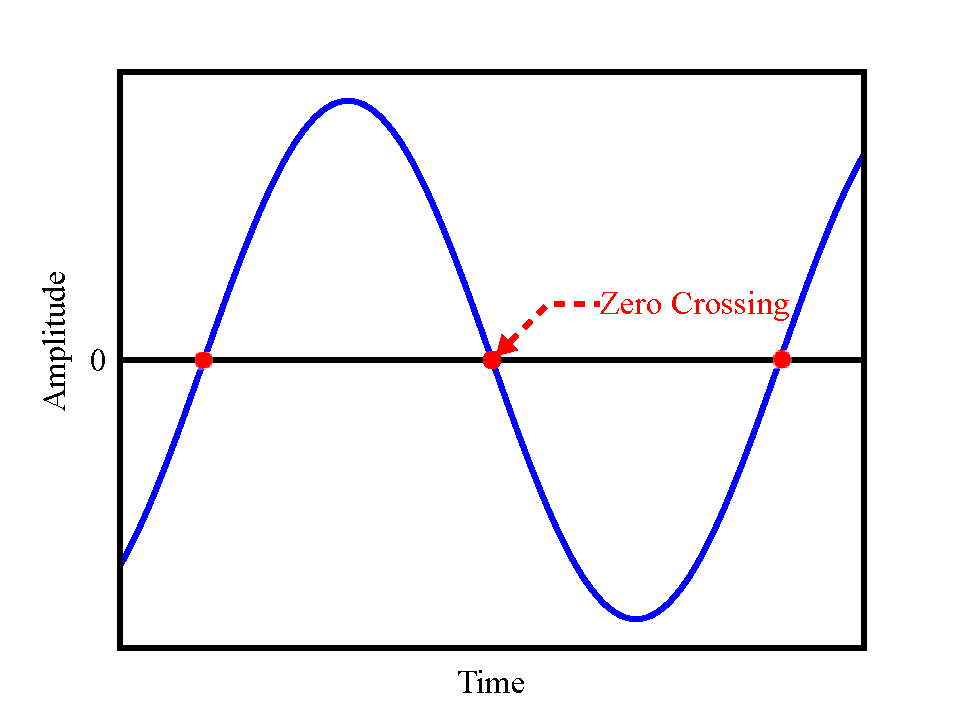
\includegraphics[width=3in]{ang/zero_crossing_illustration}
\caption{Zero Crossing Illustration (from Wikipedia)}
\label{zero_crossing_illustration}
\end{figure}

As is illustrated in Fig. \ref{zero_crossing_illustration}, a zero-crossing is a point where the \textbf{sign} of a signal changes, represented by a crossing of the time axis where amplitude is zero in the graph. Zero-crossing count is the times of zero-crossing occurrence in a stipulated period. Zero-crossing count of the $j$-th frame can be mathematically represented in (\ref{eq:frame-zcc}).

\begin{align}
\label{eq:frame-zcc}
zcc_s[j] &= \sum_{n=1}^{N-1} \Lambda ( s_j[n], s_j[n+1] )\\
\Lambda ( a, b ) &=
\begin{cases}
1, &\text{if } ab < 0\\
0, &\text{otherwise}
\end{cases}
\end{align}

%--------------------------------------------

\subsection{Features of Different Frame Types}

We manually identify the unvoiced region and voiced region (the remains are silent region) of several different words by hearing the sound and observing the waveform.

\begin{figure}[H]
\begin{minipage}[t]{0.5\linewidth}
\centering
\minipageplot{ang/threshold_example1}
\caption{Waveform, enery \& zcc}
\label{threshold_example1}
\end{minipage}
\begin{minipage}[t]{0.5\linewidth}
\centering
\minipageplot{ang/threshold_example2}
\caption{Zoomed-in Version}
\label{threshold_example2}
\end{minipage}
\end{figure}

In the case of word \textit{zero}, Fig. \ref{threshold_example1} shows the waveform and corresponding frame energy as well as the zero-crossing count of each frame. Fig. \ref{threshold_example2} is a zoomed-in version of Fig. \ref{threshold_example1}. The \textcolor{green_html}{green} dash-dot rectangle stands for the unvoiced region while the \textcolor{red}{red} dashed rectangle indicates voiced region. We can clearly see that unvoiced frames have low energy but high zero-crossing count, voiced frames have high energy but low zero-crossing count while silent frames have not only low energy but also low zero-crossing count. The relationships are summarized in Table \ref{table:thresholds}.

\begin{table}[H]
\centering
\caption{Properties of Different Frame Types}
\label{table:thresholds}
\begin{tabu} to 0.8\textwidth {XXX}
\toprule
Type &Energy &Zero-crossing count\\
\hline
Voiced &high &low\\
\hline
Unvoiced &low &high\\
\hline
Silent &low &low\\
\bottomrule
\end{tabu}
\end{table}

%--------------------------------------------

\subsection{Find Thresholds}

Fig. \ref{threshold1} shows the methods taken to find the energy threshold and the zero-crossing threshold. At the beginning, we manually identify the voiced and unvoiced frames of different words. Then, we calculate the average energy of these voiced frames and take noise level into consideration, finally determine a frame energy threshold. Analogously, we calculate the mean zero-crossing count of unvoiced frames and take the noise frequency into account, eventually obtain the zero-crossing threshold.\\

Note that thresholds are subject to the change of recording devices and environment noise. Hence, they have to be calibrated after the system is implemented on the DSP board and integrated with the \textit{Least Mean Square} noise cancellation scheme.

\begin{figure}[H]
\centering
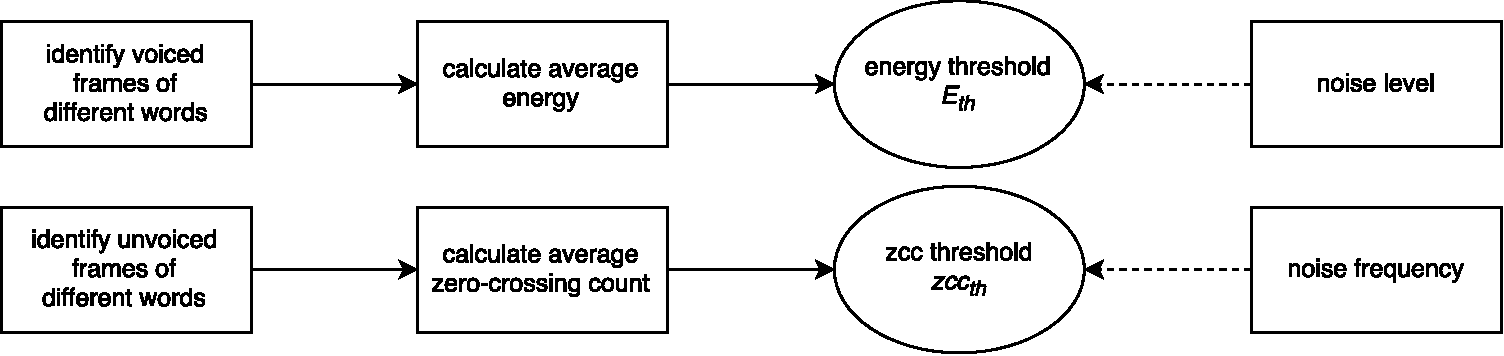
\includegraphics[width=6in]{ang/threshold1}
\caption{Methodology to Find Thresholds}
\label{threshold1}
\end{figure}

%--------------------------------------------

\subsection{Decision Rule}

Fig. \ref{threshold2} shows the decision-making strategy based on the thresholds obtained from above. Firstly, we calculate the energy of a frame and compare the energy with the threshold. A frame with higher energy is regarded as a voiced frame. Then, compute the zero-crossing count of low energy frame. If zero-crossing count is higher than the threshold, this frame is considered as unvoiced frame; otherwise, this frame will be discarded.

\begin{figure}[H]
\centering
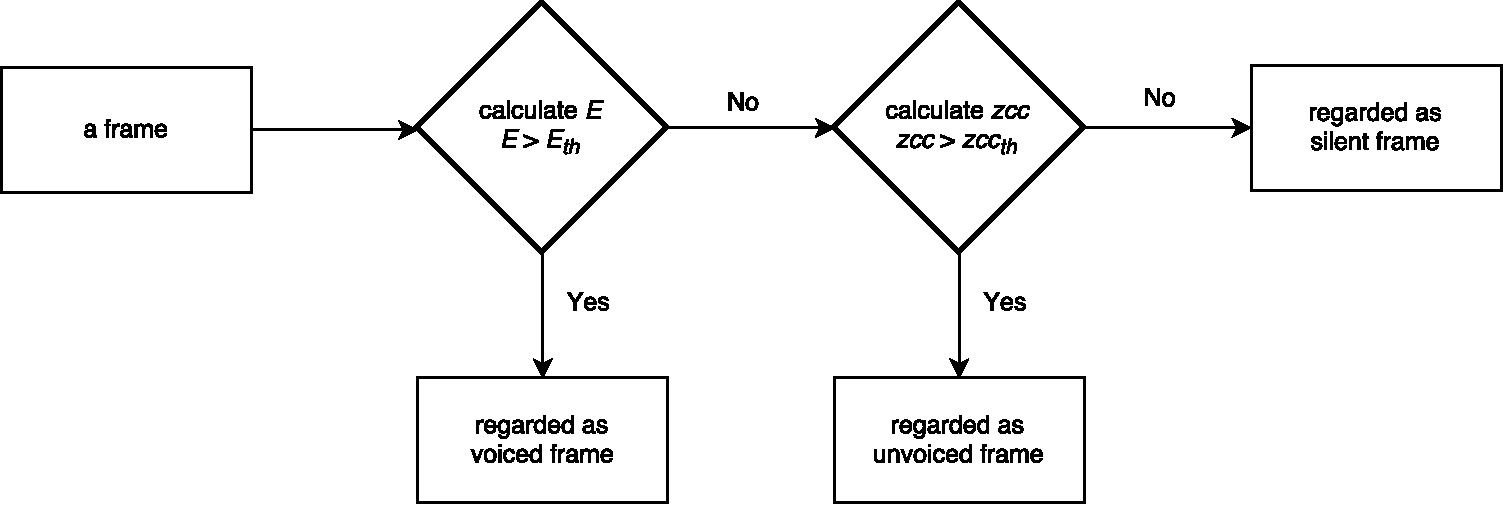
\includegraphics[width=6in]{ang/threshold2}
\caption{Decision Rule}
\label{threshold2}
\end{figure}

%--------------------------------------------
%--------------------------------------------

\section{Mel-frequency Cepstral Coefficients Extraction}
\label{subsection:mfcc}

Once informative frames are picked out by discarding the silent frames, the next stage is to calculate the Mel-frequency cepstral coefficients for each frame. MFCC algorithm is based on the concept of power cepstrum. The whole process to obtain power cepstrum defined in (\ref{eq:time-domain-to-cepstrum}) on page \pageref{eq:time-domain-to-cepstrum} can be divided into three procedures.
\begin{enumerate}
	\item Compute the Discrete Fourier Transform $S_j[k]$ and corresponding power spectrum $\hat{S}_j[k]$ of a time-domain signal $s_j[n]$.
	\item Take the logarithm of the power spectrum $\hat{S}_j[k]$.
	\item Conduct inverse Fourier transform.
\end{enumerate}

From previous section, we have known human hearing responds to the entire critical band instead of individual frequencies in this band. Thus, MFCC calculates the total power within each certain mel-scale band prior to log scaling (step 2). Moreover, MFCC substitutes Discrete Cosine Transform for inverse Fourier transform to reduce the computational complexity.

\subsection{Power Spectrum}

Discrete Fourier Transform (\ref{eq:dft}) constitutes the cornerstone of spectrum analysis.
\begin{equation}
\label{eq:dft}
S_j[k] = \sum_{n=1}^{N} s_j[n] W_N^{(n-1) k} \quad k = 1, 2, \dots, N
\end{equation}
\begin{equation}
W_N = e^{\frac{- 2\pi i}{N}}
\end{equation}

It can be clearly seen that the computations required by DFT increase dramatically as length $N$ increases. Due to the high computational requirement, direct implementation of DFT for large sequences has not been feasible. However, Fast Fourier Transform has made implementation of DFT practical in real-time processing.\\

The principles of FFT algorithms involve a divide-and-conquer approach in which an $N$-point DFT is divided into successively smaller DFTs. One of the most popular FFT algorithms is Radix-2 which restricts the sample length to a power of two. Therefore, we chose the frame length $N = 512 = 2^9$ to make full use of the FFT function. Table \ref{table:radix-2} summarizes and compares the computational requirements of DFT and Radix-2 based FFT.

\begin{table}[H]
\caption{Computational Requirements of DFT and Radix-2 FFT}
\label{table:radix-2}
\begin{tabu} to \textwidth {X[c]X[c]X[c]}
\toprule
&$N$ &$N = 512$\\
\hline
DFT multiplications &$N^2$ &262144\\
\hline
DFT additions &$N^2 - N$ &261632\\
\hline
FFT multiplications &$\frac{N}{2} \log_2(N)$ &2304\\
\hline
FFT additions &$N \log_2(N)$ &4608\\
\bottomrule
\end{tabu}
\end{table}

We have known that the DFT $X[k]$ of a real sequence $x[n]$ is a conjugate symmetric sequence (from ELEN90058 \textit{Signal Processing} Workshop 3), i.e.
\begin{equation}
X[k] = X^*[\langle-k\rangle_{N}] = X^*[N-k]
\end{equation}

When computing the power spectrum, we are motivated to use this symmetry property and discard the last $(\frac{N}{2} - 1)$ points. Specifically, $S_j[1]$ is DC component of the signal; $S_j[2]$ to $S_j[\frac{N}{2}]$ are the first half of the complex spectrum; $S_j[\frac{N}{2} + 1]$ is the component at Nyquist frequency (8000 Hz).
\begin{equation}
\label{eq:power-spectrum}
\hat{S}_j[k] = |S_j(k)|^2 \quad k = 1, 2, \dots, \frac{N}{2} + 1
\end{equation}

%--------------------------------------------

\subsection{Bank Filtering}

The energy within each mel-scale bank can be computed by (\ref{eq:mel-filter}).
\begin{equation}
\label{eq:mel-filter}
X_j[m] = \sum^{\frac{N}{2} + 1}_{k=1} \hat{S}_j[k] H_{mel}[m, k]
\end{equation}
where $H_{mel}[m, k]$ is the gain of $k$-th power data point within bank $m$ and $m = 1, 2, \dots, M$.\\

\begin{equation}
\label{eq:mel-bank-gain}
H_{mel}[m, k] =
\begin{cases}
0 &f_{d2c}(k) \le f[m-1]\\
\displaystyle\frac{k - f[m-1]}{f[m] - f[m-1]} &f[m-1] < f_{d2c}(k) \le f[m]\\
\displaystyle\frac{f[m+1] - k}{f[m+1] - f[m]} &f[m] < f_{d2c}(k) \le f[m+1]\\
0 &f_{d2c}(k) > f[m+1]
\end{cases}
\end{equation}
where $f_{d2c}(k) = (k-1) \cdot \frac{F_s}{N}$ transforms the DFT data point into continuous-time frequency.

$f[m] \in [0, 8000]$ Hz are equally spaced in the mel-scale and can be computed by (\ref{eq:bank-boundary}). We take $f_{\min}$ = 1 Hz and $f_{\max} = \frac{F_s}{2}$ = 8000 Hz as per the system specification and $M = 20$ according to \cite{davis1980comparison}.
\begin{equation}
\label{eq:bank-boundary}
f[m] = \mel^{-1} \left( \mel(f_{\min}) + m \cdot \frac{\mel(f_{\max}) - \mel(f_{\min})}{M + 1} \right)
\end{equation}
where $m = 0, 1, \dots, M+1$ and the mel-scale to frequency transform $\mel^{-1}(f_{mel})$ is the inverse function of (\ref{eq:mel-function}).
\begin{equation}
\label{eq:mel-function-inverse}
f = \mel^{-1}(f_{mel}) = 700 \left( 10^{\left(\frac{f_{mel}}{2595}\right)} - 1 \right); \quad f \text{ in Hz}
\end{equation}

\begin{figure}[H]
\centering
\wideplot{ang/mel_triangle}
\caption{Mel Filter Banks}
\label{mel_triangle}
\end{figure}

Fig. \ref{mel_triangle} shows that $H_{mel}$ given in (\ref{eq:mel-bank-gain}) and (\ref{eq:bank-boundary}) is essentially a band-pass filter for each bank. $H_{mel}$ offers maximal gain 1 at $f[m]$ (the `central frequency' of this bank in mel-scale) and then linearly decreases to 0 until reaching adjacent frequency boundaries ($f[m-1]$ and $f[m+1]$) on both sides.\\

Fig. \ref{bank_filter_demostration} depicts the process to compute $X_j[m]$ of bank $m = 9$ based on (\ref{eq:mel-filter}). In subplot 1, each power data point $\hat{S}_j[k]$ (\textcolor{gold_matlab}{gold circle $\circ$}) is multiplied by the corresponding gain $H_{mel}[m, k]|_{m=9}$ (\textcolor{orange_matlab}{orange asterisk $*$}). Filtered power data points are shown in subplot 2 by \textcolor{orange_matlab}{orange cross $\times$}. Thereby, the sum of all filtered power data points is the energy $X_j[m]$ within filter bank $m = 9$.

\begin{figure}[H]
\begin{minipage}[t]{0.5\linewidth}
\centering
\minipageplot{ang/bank_filter_demostration}
\caption{Bank Filtering Demonstration}
\label{bank_filter_demostration}
\end{minipage}
\begin{minipage}[t]{0.5\linewidth}
\centering
\minipageplot{ang/mel_filter_bank_gain}
\caption{Gain of Each Point in Each Bank}
\label{mel_filter_bank_gain}
\end{minipage}
\end{figure}

(\ref{eq:power-spectrum}) can be further simplified because $H_{mel}[m, 0]$ = $H_{mel}[m, \frac{N}{2}+1] = 0$, $\forall m = 1, 2, \dots, M$. Fig. \ref{mel_triangle} also visualizes this property. Hence, only the first half of the \textbf{complex} spectrum need to be taken into consideration when computing power spectrum.
\begin{equation}
\hat{S}_j[k] = |S_j(k)|^2 \quad k = 2, \dots, \frac{N}{2}
\end{equation}

%--------------------------------------------

\subsection{Log Scaling}

\begin{equation}
\label{eq:log-scaling}
\hat{X}_j[m] = \log_{10}(X_j[m]) \quad m = 1, 2, \dots, M
\end{equation}

%--------------------------------------------

\subsection{Discrete Cosine Transform}

\begin{equation}
\label{eq:dct}
\hat{C}_j[n] = w_{dct}[n] \sum^{M}_{m=1} \hat{X}_j[m] \cos \left( \frac{\pi}{M} (m - 0.5) (n-1) \right) \quad n = 1, 2, \dots, F
\end{equation}
where
\begin{equation}
\label{eq:dct-weight}
w_{dct}[n] = \sqrt{\frac{2}{M}}
\end{equation}

\chapter{Hidden Markov Model}

\chapter{Digital Signal Processor}
\label{chapter:dsp}

%----------------------------------------------------------------------------------------
%	Section
%----------------------------------------------------------------------------------------

\section{ADSP-BF548 EZ-KIT Lite}

This section primarily summarizes the hardware-related information that helps developers write more robust and efficient C code.

%--------------------------------------------
%--------------------------------------------

\subsection{Hardware Architecture}

\textbf{Audio Codec} in charge of sampling speech and \textbf{Memory Hierarchy} that restricts the storage of variables are highly significant to the implementation on the DSP board.

%--------------------------------------------

\subsubsection{Audio Codec}
An Analog Devices AD1980 audio codec is the audio interface of the EZ-KIT Lite. The codec connects to multiple audio connectors (3.5 mm) which allow us to get audio in and out. These connectors can be easily found at the bottom left corner of the board.

\begin{figure}[H]
\centering
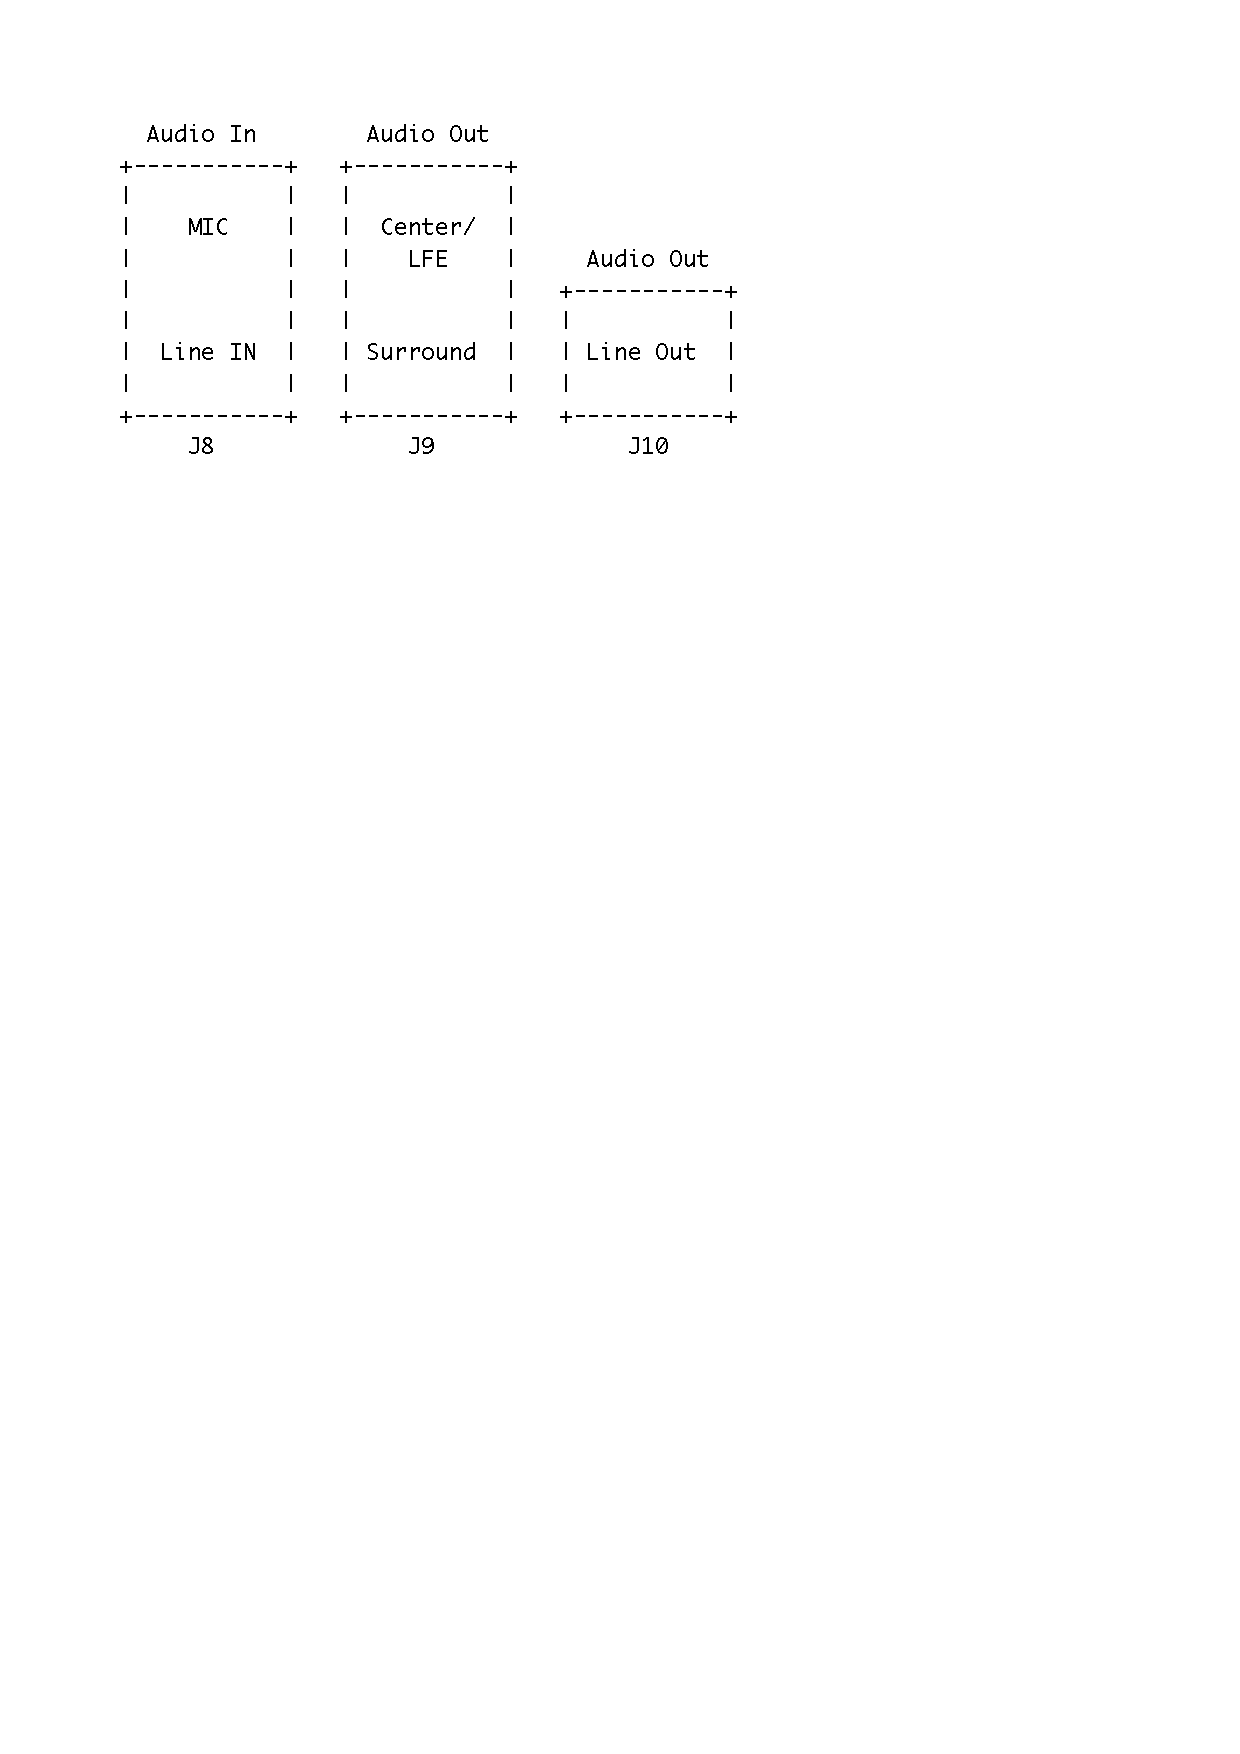
\includegraphics[width=3in]{ang/audio-connectors}
\caption{Audio Connectors}
\label{audio-connectors}
\end{figure}

Fig. \ref{audio-connectors} illustrates that the top location of \texttt{J8} is for a stereo microphone and the bottom location is for a stereo line in. According to Fig. \ref{AD1980-schematic}, the difference between \texttt{MIC} and \texttt{LINE IN} is signals via \texttt{MIC} will be pre-amplified. The preamp gain is collaboratively controlled by \texttt{MIC} Volume Register (\texttt{AD1980\_REG\_MIC\_VOL\_CTRL}) and Miscellaneous Control Bit Register (\texttt{AD1980\_REG\_MIC\_VOL\_CTRL}) \cite{AC97-codec}. In addition, it can be clearly seen that AD1980 can only sample 2 channels at any given moment due to the RECORD SELECTOR multiplexer. Thus, we decide to input noisy command and noise via the left / right channel of \texttt{MIC} respectively.

\begin{figure}[H]
\centering
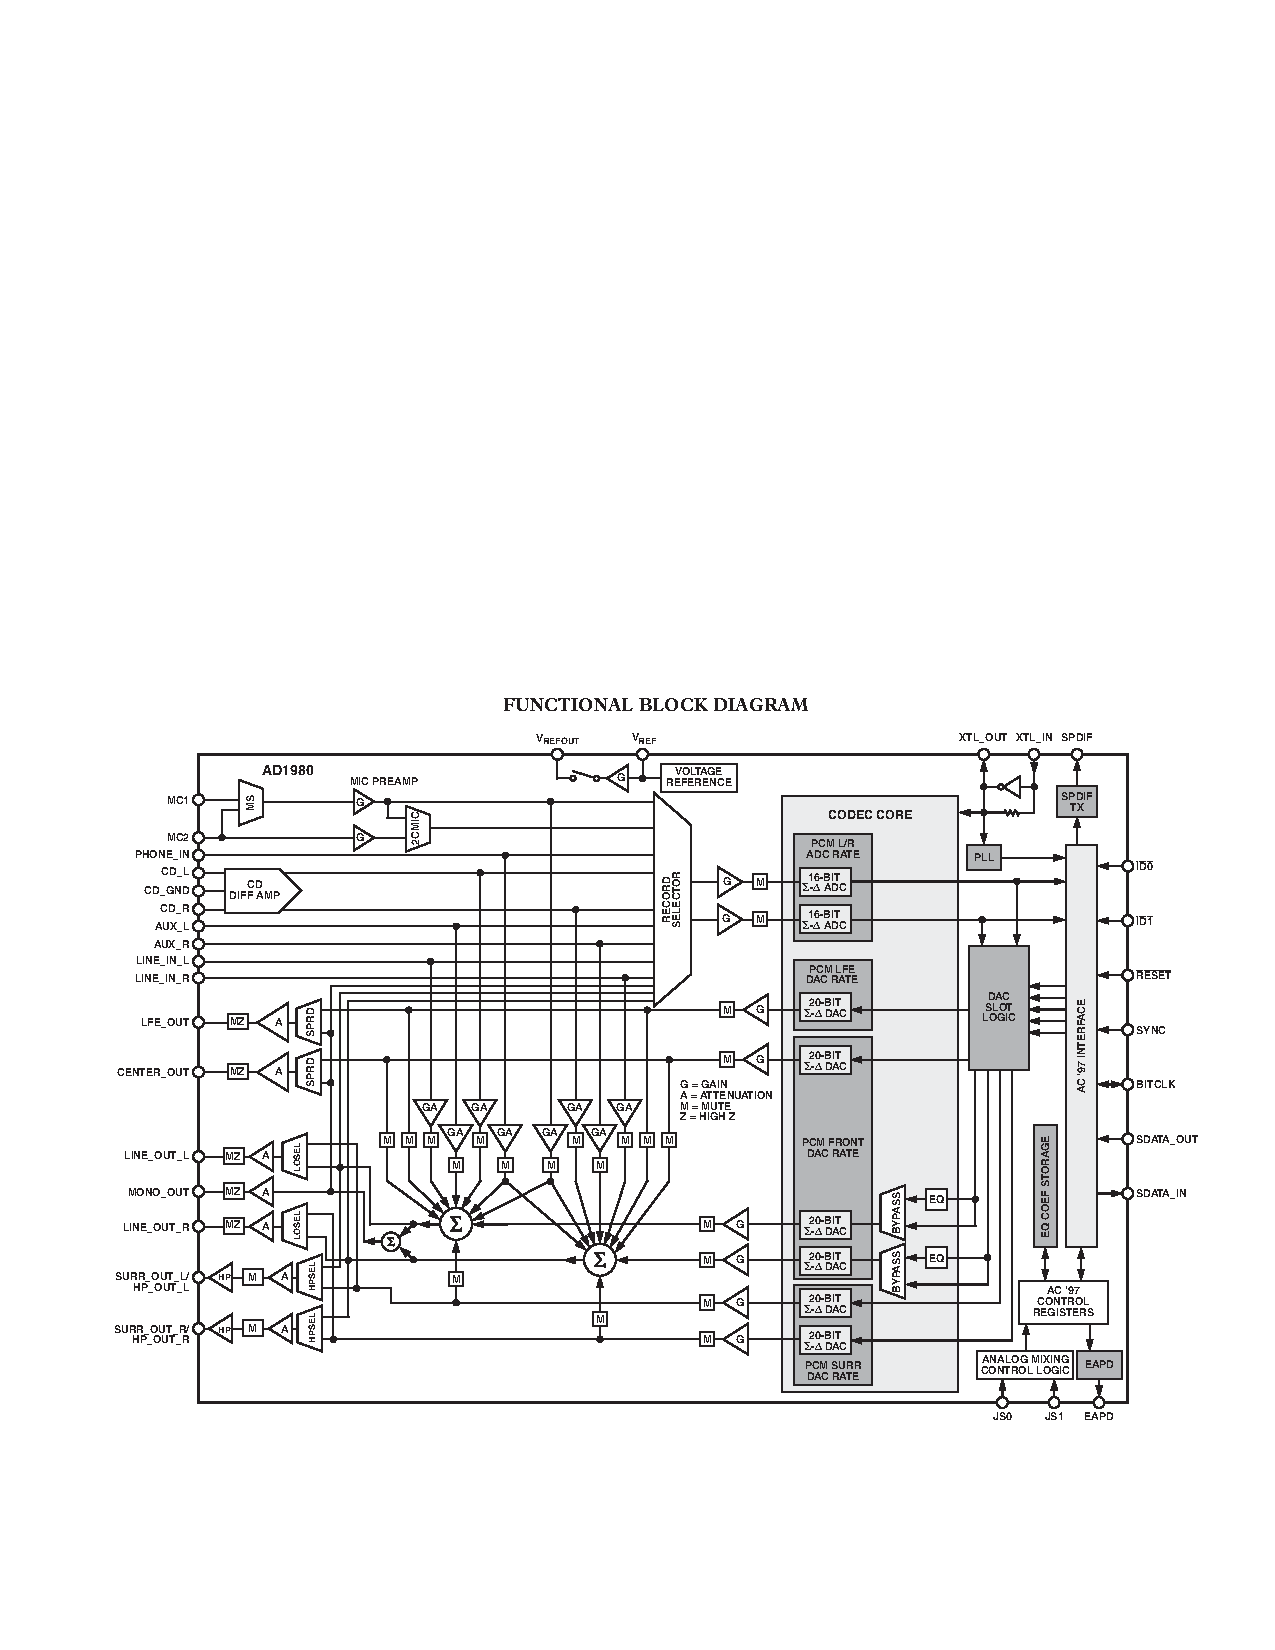
\includegraphics[width=6in]{ang/AD1980-schematic}
\caption{AD1980 Functional Block Diagram}
\label{AD1980-schematic}
\end{figure}

%--------------------------------------------

\subsubsection{Memory Hierarchy}
The ADSP-BF548 processor supports a hierarchy of three synchronous memories.\\

Internal L1 memory offers two 32 KB SRAM banks for data \cite{bf54x-hardware}. ``L1 memory is the highest-performing memory available to the Blackfin core and can be accessed at core clock speeds.''\cite{start-with-bf548}\\

Internal L2 memory consists of a single 128 KB area of SRAM. ``L2 is somewhat lower-performing than L1, requiring two core clock cycles for access.'' L2 provides larger capacity accompanied by higher latency. \cite{start-with-bf548} Totally, 32768 variables of 32-bit data type (e.g. \texttt{float} and \texttt{fract32}) can be stored in L2.\\

External memory is a 64 MB DDR SDRAM that exists external to the processor mounted on the DSP board. ``External memory operates synchronously with the processor's system clock rather than the core clock, causing access time to SDRAM to be relatively slower than to L1 or L2 memory.''\cite{start-with-bf548} 64 MB (67108864 bytes) is enormous given that each \texttt{float} / \texttt{fract32} variable occupies 4 bytes. Hence, we will pre-compute reusable coefficients as long as fetching them from external memory is faster than computing them. In fact, L1 \& L2 are big enough to store these coefficients, decisions will be elaborated in \fullref{section:c_program}.

%--------------------------------------------
%--------------------------------------------

\subsection{Data Types}

\subsubsection{Directly Supported Data Types}

Table \ref{fixed-point-data-types} (in appendix on page \pageref{fixed-point-data-types}) and Table \ref{floating-point-data-types} summarize the ten scalar data types directly supported by the complier.\\

Table \ref{main-fixed-point-data-types} as a subset of Table \ref{fixed-point-data-types} lists main fixed-point data types. Note that \texttt{long} is equivalent to \texttt{int}. We use 8-bit \texttt{unsigned char} when manipulating GPIO (\textit{General Purpose I/O}) registers.

\begin{table}[H]
\centering
\caption{Main Fixed-Point Data Types}
\label{main-fixed-point-data-types}
\begin{tabu} to \textwidth {XXXX}
\toprule
Type &Size &Min &Max\\
\hline
\texttt{unsigned char} &8-bit &0 &255\\
\hline
\texttt{short} &16-bit &-32,768 &32,767\\
\hline
\texttt{int} &32-bit &-2,147,483,648 &2,147,483,647\\
\hline
\texttt{long} &32-bit &-2,147,483,648 &2,147,483,647\\
\bottomrule
\end{tabu}
\end{table}

Table \ref{floating-point-data-types} summarizes properties of floating-point data types. Note that \texttt{double} is equivalent to \texttt{float}. Value ranges are computed based on the internal representation of single-precision floating-point numbers. Details are provided in appendix on page \pageref{subsection:float-data-type}. We have also shown \texttt{float} has a precision of $\log_{10}(2^{24}) \approx 7.225$ decimal digits in the appendix. This deduction is significant to exporting model and coefficients from MATLAB.

\begin{table}[H]
\centering
\caption{Floating-Point Data Types}
\label{floating-point-data-types}
\begin{tabu} to \textwidth {XXX}
\toprule
Type &Size &Range\\
\hline
\texttt{float} &32-bit &$\pm 1.18 \times 10^{-38}$ to $\pm 3.4 \times 10^{38}$\\
\hline
\texttt{double} &32-bit &$\pm 1.18 \times 10^{-38}$ to $\pm 3.4 \times 10^{38}$\\
\bottomrule
\end{tabu}
\end{table}

The smallest denormalized number has a marked impact on small probability calculation. For instance, the emission probability can easily become smaller than $e^{-200} = 1.3839 \times 10^{-87}$. Fortunately, all computation involved between probabilities are multiplications, hence we take natural logarithm before conducting multiplications and convert all multiplications into additions based on the property of logarithm (\ref{log-property}).

\begin{equation}
\label{log-property}
\ln(xy) = \ln(x) + \ln(y)
\end{equation}

%--------------------------------------------

\subsubsection{Fractional Data Types}

Fractional data types \texttt{fract16} and \texttt{fract32} can be represented as \texttt{short} and \texttt{int} respectively. Fig. \ref{bf_fract_represent} shows the internal representation of \texttt{fract16} and \texttt{fract32} (from National Instruments). The properties of fractional data types are listed in Table \ref{fractional-data-types}.

\begin{figure}[H]
\centering
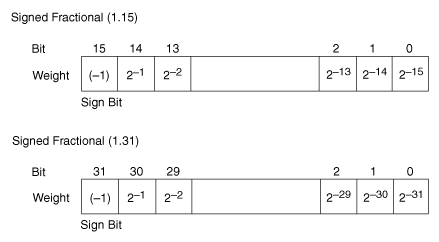
\includegraphics[width=3in]{ang/bf_fract_represent}
\caption{Internal Representation of Fractional Data Types}
\label{bf_fract_represent}
\end{figure}

\begin{table}[H]
\centering
\caption{Fractional Data Types}
\label{fractional-data-types}
\begin{tabu} to \textwidth {XXXX}
\toprule
Type &Size &Range &Resolution\\
\hline
\texttt{fract16} &16-bit &$-1$ to $1 - 2^{-15}$ &$2^{-15}$\\
\hline
\texttt{fract32} &32-bit &$-1$ to $1 - 2^{-31}$ &$2^{-31}$\\
\bottomrule
\end{tabu}
\end{table}

%--------------------------------------------
%--------------------------------------------

\subsection{CrossCore Embedded Studio}

During ELEN90058 \textit{Signal Processing} and ELEN90052 \textit{Advanced Signal Processing} workshop sessions, we used CrossCore\textsuperscript{\textregistered} Embedded Studio to compile and debug code for Blackfin DSP board. Basing on Eclipse, CCES exploits the ecosystem of third-party tools already available to Eclipse developers. Thus, plenty of convenient functions such as plotting arrays of data are available to users \cite{erik-cces}\cite{cces-faq}. CCES could be an ideal substitution for VisualDSP++.\\

However, the AD1980 Audio Codec on ADSP-BF548 EZ-Kit Lite Board is not supported with CCES \cite{cces-ad1980}. Analog Devices engineer Craig Gilchrist explained in \textit{EngineerZone} support community that they do not have a driver for the AD1980 Codec with CCES. In addition, he recommended AD1836 Audio Codec instead \cite{BF548-BSP}.\\

Considering the project budget and potential risk, we eventually decided to stick on VisualDSP++ 5.1.2.

%----------------------------------------------------------------------------------------
%	Section
%----------------------------------------------------------------------------------------

\section{Software Development}

\subsection{Software Process}
We develop the software system of our project according to the following set of activities.
\begin{enumerate}
\item Determine system specification.
\item Design algorithm in MATLAB.
\item Optimize program efficiency in MATLAB, e.g. pre-computing reusable coefficients, taking advantage of symmetry, scaling data in order to use fixed-point arithmetic.
\item Develop evolutionarily. Implementation and validation are interleaved.
\begin{enumerate}
	\item Implement each function in C language on DSP board.
	\item Validate each function by comparing the outcomes calculated by DSP with the expected results from MATLAB. Round off errors are allowed but differences are supposed to be within precision tolerance.
\end{enumerate}
\item Adjust algorithm in MATLAB if the original design is infeasible to implement due to precision and speed restriction of DSP board.
\item Implement algorithms for real-time processing.
\item Tune performance by optimizing efficiency and improving accuracy.
\end{enumerate}

%--------------------------------------------
%--------------------------------------------

\subsection{Revision Control \& Source Code Management}

We host and manage our code on GitHub which helps us control revisions and manage source code better. Reviewing what has been modified before committing the change to the server minimizes the possibility of misoperation. Besides, we hope our work could contribute to the open-source community inversely because we have benefited from open-source spirit so much.\\

Project Repository: \url{https://github.com/leeang/Word-Recognition}

%----------------------------------------------------------------------------------------
%	Section
%----------------------------------------------------------------------------------------

\section{C Program}
\label{section:c_program}

In addition to the experience gained in workshops, \cite{TuningCSourceCode} provides official guidance for optimizing C program execution efficiency. During implementation, we reduce floating-point arithmetic as much as possible and try to avoid integer division in loops.

\subsection{Audioloopback}

%--------------------------------------------
%--------------------------------------------

\subsection{Pre-emphasis}

It is easy to prove that filter characteristic represented by (\ref{shelving-filter}) will not change if coefficients $a_i$ and $b_i$ are uniformly scaled. Some pre-emphasis filter coefficients (\ref{shleving-coef}) are beyond the fractional data types domain $[-1, 1]$. Hence, the coefficients are scaled by $\lambda$ before converting them from \texttt{float} to \texttt{fract32}.\\

We choose $\lambda = \frac{1}{4}$ primarily because $\frac{1}{a_0} = \frac{1}{\lambda} = 4$ which is a power of 2. In terms of fixed-point data types, left shifting 2 bits is equivalent to multiplying by $\frac{1}{a_0} = 4$ but left shifting is more efficient. Besides, $\lambda = \frac{1}{2}$ is not small enough while $\lambda = \frac{1}{8}$ leads to loss in precision. $a_i \in [-1, 1]$ and $b_i \in [-1, 1]$ for $\forall i = 0, 1, 2$ when $\lambda = \frac{1}{4}$.

\begin{align*}
&\begin{cases}
a_0 = \frac{1}{4} = 0.25\\
a_1 = \frac{-1.523796}{4} = -0.380949\\
a_2 = \frac{0.649345}{4} = 0.162336
\end{cases}
&\begin{cases}
b_0 = \frac{1.861856}{4} = 0.465464\\
b_1 = \frac{-3.102851}{4} = -0.775712\\
b_2 = \frac{1.366544}{4} = 0.341636
\end{cases}
\end{align*}

Filter coefficients are converted into \texttt{fract32} once by \texttt{calc\_shelving\_coef()} function when initializing the system. Finally, all computations in \texttt{pre\_emphasis()} function are fixed-point arithmetic.

%--------------------------------------------
%--------------------------------------------

\subsection{Hamming Window}

For the window length $N = 512$, Hamming window weight $w[n]$ has 512 elements. Table \ref{clocks-hamming} summarizes the efficiency of different methods to obtain $w[n]$. $512/2 = 256$ (due to symmetry) \texttt{fract32} data points occupy 1 KB. There is no reason to recompute them every time. Considering they are most frequently used (180 times per 3-second recording), we store them in the fastest L1 memory. During the initialization session, \texttt{calc\_hamming\_coef} function pre-computes them and converts them into \texttt{fract32}. All computations in \texttt{hamming()} function are fixed-point arithmetic.

\begin{table}[H]
\centering
\caption{Efficiency of Approaches to Obtain $w[n]$}
\label{clocks-hamming}
\begin{tabu} to \textwidth {XXX}
\toprule
Action &clocks &time elapsed\\
\hline
compute &607471 &1.012452 ms\\
\hline
fetch from L1 &8731 &0.014552 ms\\
\hline
fetch from L2 &12827 &0.021378 ms\\
\hline
fetch from external memory &30878 &0.051463 ms\\
\bottomrule
\end{tabu}
\end{table}

From (\ref{eq:windowing}), we have
\begin{equation}
s_j[n] = w[n] s[n+jN] \quad n = 1, 2, \dots, N
\end{equation}
We have known $|s[n+jN]| \le 1$, thus
\begin{equation}
|s_j[n]| = |w[n]| \cdot |s[n+jN]| \le |w[n]| \quad n = 1, 2, \dots, N
\end{equation}
\begin{equation}
\Longrightarrow |s_j[n]|^2 \le |w[n]|^2 \quad n = 1, 2, \dots, N
\end{equation}
\begin{equation}
\Longrightarrow \sum_{n=1}^{N} |s_j[n]|^2 \le \sum_{n=1}^{N} |w[n]|^2
\end{equation}

Based on (\ref{eq:hamming}), for Hamming window length $N = 512$,
\begin{equation}
\sum_{n=1}^{N} |w[n]|^2 = 203.0778 < 256
\end{equation}

Hence,
\begin{equation}
\label{hamming-inequation}
\sum_{n=1}^{N} |s_j[n]|^2 \le \sum_{n=1}^{N} |w[n]|^2 < 256
\end{equation}

%--------------------------------------------
%--------------------------------------------

\subsection{Thresholds}
\subsubsection{Frame Energy}

From (\ref{eq:frame-energy}) and (\ref{hamming-inequation}), we have
\begin{align}
\label{energy-inequation}
&E_s[j] = \sum_{n=1}^{N} |s_j[n]|^2 < 256\\
&\Longrightarrow \sum_{n=1}^{N} \frac{1}{256} |s_j[n]|^2 < 1
\end{align}

(\ref{energy-inequation}) shows that the frame energy will not overflow if we scale the square of amplitudes by $\frac{1}{256}$ before accumulation. Right-shifting the square of amplitudes by $\log_2(256) = 8$ bits is equivalent to multiplying by $\frac{1}{256}$.\\

Right-shifting leads to loss in precision. However, we calculate frame energy only for comparison with the threshold, i.e. the exact value will not be used in further computations, thus the error will not be accumulated. In addition, the change of recording device and environment voice influence much more than the error caused by right-shifting.\\

\texttt{calc\_energy()} function calculates the scaled energy of a frame. Note that the energy threshold should be scaled by $\frac{1}{256}$ before converted into \texttt{fract32} data type during system initialization. Finally, all computations and comparisons related to frame energy are fixed-point arithmetic.

%--------------------------------------------
%--------------------------------------------

\subsection{MFCC extraction}
\subsubsection{Power Spectrum}

We have known that the DFT of a $N$-point real sequence can be obtained from one $\frac{N}{2}$-point complex-valued DFT and additional computations (from ELEN90058 \textit{Signal Processing} lecture slides by Erik \textsc{Weyer}). VisualDSP++ has a built-in function called \texttt{rfft\_fr32()} to exploit this property.\\

\texttt{rfft\_fr32()} function takes 7 arguments. The first two are time domain real sequence input and spectrum output. The third one is the twiddle table calculated once by \texttt{twidfftrad2\_fr32()} function during system initialization. The fourth parameter is the twiddle stride that should be set to 1 because the twiddle table is tailored to this FFT. The fifth argument is the FFT size which equals the window length $N = 512$. The last two are block exponent and scaling method. We select dynamic scaling mode that will inspect intermediate results and only apply scaling where required to prevent overflow. In this mode, precision can be better preserved than in static scaling method, although inspections leads to an negative impact on performance. The block exponent returned will be the number of times that the function scales the intermediate set of results.\\

Once the spectrum is obtained, we invoke \texttt{cabs\_fr32()} function to compute the magnitude of each data point (data type: \texttt{complex\_fract32}), the product of the magnitude and itself is the power of each point.

%--------------------------------------------

\subsubsection{Bank Filtering \& Log Scaling}

Fig. \ref{bank_filter_demostration} depicts the process to compute $X_j[m]$ of bank $m = 9$ based on (\ref{eq:mel-filter}) on page \pageref{eq:mel-filter}. In subplot 1, each power data point $\hat{S}_j[k]$ (\textcolor{gold_matlab}{gold circle $\circ$}) is multiplied by the corresponding gain $H_{mel}[m, k]|_{m=9}$ (\textcolor{orange_matlab}{orange asterisk $*$}). Filtered power data points are shown in subplot 2 by \textcolor{orange_matlab}{orange cross $\times$}. Thereby, the sum of all filtered power data points is the energy $X_j[m]$ within filter bank $m = 9$.

\begin{figure}[H]
\begin{minipage}[t]{0.5\linewidth}
\centering
\minipageplot{ang/bank_filter_demostration}
\caption{Bank Filtering Demonstration}
\label{bank_filter_demostration}
\end{minipage}
\begin{minipage}[t]{0.5\linewidth}
\centering
\minipageplot{ang/mel_filter_bank_gain}
\caption{Gain of Each Point in Each Bank}
\label{mel_filter_bank_gain}
\end{minipage}
\end{figure}

Fig. \ref{bank_filter_demostration} also shows that bank $m=9$ only intersects with 16 data points in power spectrum because gain for other points are all zero. We plot the gain of each data point for each bank in Fig. \ref{mel_filter_bank_gain}, grayscale represents the value of gain. We find the same situation for all banks. Directly computing $H_{mel}[m, k]$ results in a $k \times m$ sparse matrix (white blocks stand for zeros).\\

In order to diminish the processing time by pre-computing and eliminating the useless operations with zeros, we design a special storage structure for this sparse matrix. One array for storing non-zero values in linear shape and one array for storing corresponding offset for each bank. One array for storing at which $k$ gain becomes non-zero (\textcolor{red}{red dashed-line arrows}) and one-array for storing the length of each grayscale block (\textcolor{orange_html}{orange solid-line arrows}).\\

Gains are converted into \texttt{fract32} by \texttt{calc\_bank\_gain()} function during system initialization. Power cepstrum data points are converted back to \texttt{float} in case of overflow before accumulation that evaluates the total power within each bank.  We did not scale data as we had done when calculating frame energy, because
\begin{enumerate}
\item only 30 - 50 frames (out of 180 frames) are passed to MFCC;
\item precision error will be accumulated;
\item log scaling in the next step will be done with the aid of \texttt{float} type \texttt{log()} function.
\end{enumerate}

%--------------------------------------------

\subsubsection{Discrete Cosine Transform}

We define
\begin{equation}
\label{eq:dct-coef}
H_{dct}[n, m] = \sqrt{\frac{2}{M}} \cos \left( \frac{\pi}{M} (m - 0.5) (n-1) \right)
\end{equation}
where $n = 1, 2, \dots, F$ and $m = 1, 2, \dots, M$.\\

Thereby, (\ref{eq:dct}) becomes
\begin{equation}
\label{eq:dct-coef-form}
\hat{C}_j[n] = \sum^{M}_{m=1} \hat{X}_j[m] H_{dct}[n, m] \quad n = 1, 2, \dots, F
\end{equation}

It can be proven that for even $M$ and odd $F$
\begin{equation}
H_{dct}[n, m] =
\begin{cases}
H_{dct}[n, M-m+1] & n = 1, 3, \dots, F\\
-H_{dct}[n, M-m+1] & n = 2, 4, \dots, F-1
\end{cases}
\end{equation}

By utilizing this symmetry, (\ref{eq:dct-coef-form}) can be simplified as
\begin{equation}
\label{eq:dct-symmetric-form}
\hat{C}_j[n] = 
\begin{cases}
\displaystyle\sum^{M/2}_{m=1} (\hat{X}_j[m] + \hat{X}_j[M-m+1]) H_{dct}[n, m] & n = 1, 3, \dots, F\\
\displaystyle\sum^{M/2}_{m=1} (\hat{X}_j[m] - \hat{X}_j[M-m+1]) H_{dct}[n, m] & n = 2, 4, \dots, F-1
\end{cases}
\end{equation}

To calculate $\hat{C}_j[n]$ for each $n$, (\ref{eq:dct-coef-form}) requires $M$ multiplications and $(M - 1)$ additions while (\ref{eq:dct-symmetric-form}) requires $M/2$ multiplications (reduced by 50\%) and $(M - 1)$ additions. Furthermore, only a half pre-computed coefficients need to be stored in memory.\\

We pre-compute $H_{dct}[n, m]$ by \texttt{calc\_dct\_coef()} while initializing the system. Table \ref{clocks-dct} summarizes the efficiency of different methods to obtain $H_{dct}[n, m]$. It can be clearly seen that fetching from external memory is even 40 times faster than directly computing.

\begin{table}[H]
\centering
\caption{Efficiency of Approaches to Obtain $H_{dct}[n, m]$}
\label{clocks-dct}
\begin{tabu} to \textwidth {XXX}
\toprule
Action &clocks &time elapsed\\
\hline
compute &172281 &0.287135 ms\\
\hline
fetch from L1 &3889 &0.006482 ms\\
\hline
fetch from L2 &4929 &0.008215 ms\\
\hline
fetch from external memory &9367 &0.015612 ms\\
\bottomrule
\end{tabu}
\end{table}

%----------------------------------------------------------------------------------------
%	Section
%----------------------------------------------------------------------------------------

\section{Improvements on previous work}

\begin{enumerate}
\item first-order FIR pre-emphasis filter is replaced by shelving filter.
\item coefficients that intensively require floating-point computations are pre-computed.\\(pre-emphasis, Hamming window and discrete cosine transform)
\item frame energy is calculated in fixed-point arithmetic.
\item Mel bank filter gains are pre-computed and stored in an ingeniously designed structure. Meaningless multiplications with zeros are illuminated.
\end{enumerate}

%----------------------------------------------------------------------------------------
%	Section
%----------------------------------------------------------------------------------------

\section{Performance}

\subsection{Feature Extraction \& Recognition}

It takes 107.851525 ms (64710920 clocks) to process 48000 data points from pre-emphasis to recognition result.\\

Fig. \ref{probability_comparison_1} compares the probabilities of 27 words computed by MATLAB and DSP: no apparent difference can be seen. In fact, the relative error defined in (\ref{eq:relative_error}) is of the order of magnitude of $10^{-5}$ as shown in Fig. \ref{probability_error_1}.

\begin{equation}
\label{eq:relative_error}
\text{relative error} = \frac{\text{result from DSP} - \text{result from MATLAB}}{\text{result from MATLAB}}
\end{equation}

\begin{figure}[H]
\begin{minipage}[t]{0.5\linewidth}
\centering
\minipageplot{ang/probability_comparison_1}
\caption{Result Comparison}
\label{probability_comparison_1}
\end{minipage}
\begin{minipage}[t]{0.5\linewidth}
\centering
\minipageplot{ang/probability_error_1}
\caption{Relative Error of Probabilities}
\label{probability_error_1}
\end{minipage}
\end{figure}

\section{Design \& Performance}

\begin{frame}
\frametitle{Frame Title}
\end{frame}

\section{Final Implementation}

%----------------------------------------------------------------------------------------
%	Subsection
%----------------------------------------------------------------------------------------

\begin{frame}
\frametitle{Improvements on previous work}
\begin{enumerate}
	\item Coefficients that intensively require floating-point computations are precomputed.
	\begin{itemize}
		\item Hamming window, Mel-bank filter gain, discrete cosine transform
	\end{itemize}
	\item Sparse matrices are stored in ingeniously designed structures. Meaningless multiplications with zeros are illuminated.
	\begin{itemize}
		\item Mel bank filter gain, inversed variance matrices, transition matrices
	\end{itemize}
	\item Symmetry is sufficiently taken in to consideration.
	\begin{itemize}
		\item FFT of real sequence, discrete cosine transform
	\end{itemize}
\end{enumerate}

\begin{itemize}
\item Hamming window: $1 - \frac{0.014552 \text{ ms}}{1.012452 \text{ ms}} = 99\%$
\item DCT: $1 - \frac{0.006482 \text{ ms}}{0.287135 \text{ ms}} = 98\%$
\end{itemize}
\end{frame}

%--------------------------------------------

\begin{frame}
Feature Extraction \& Recognition
\begin{itemize}
\item The average processing time of these 23 datasets is 95.8 ms.
\item The maximal processing time is 150 ms.
\end{itemize}

\begin{figure}[H]
\centering
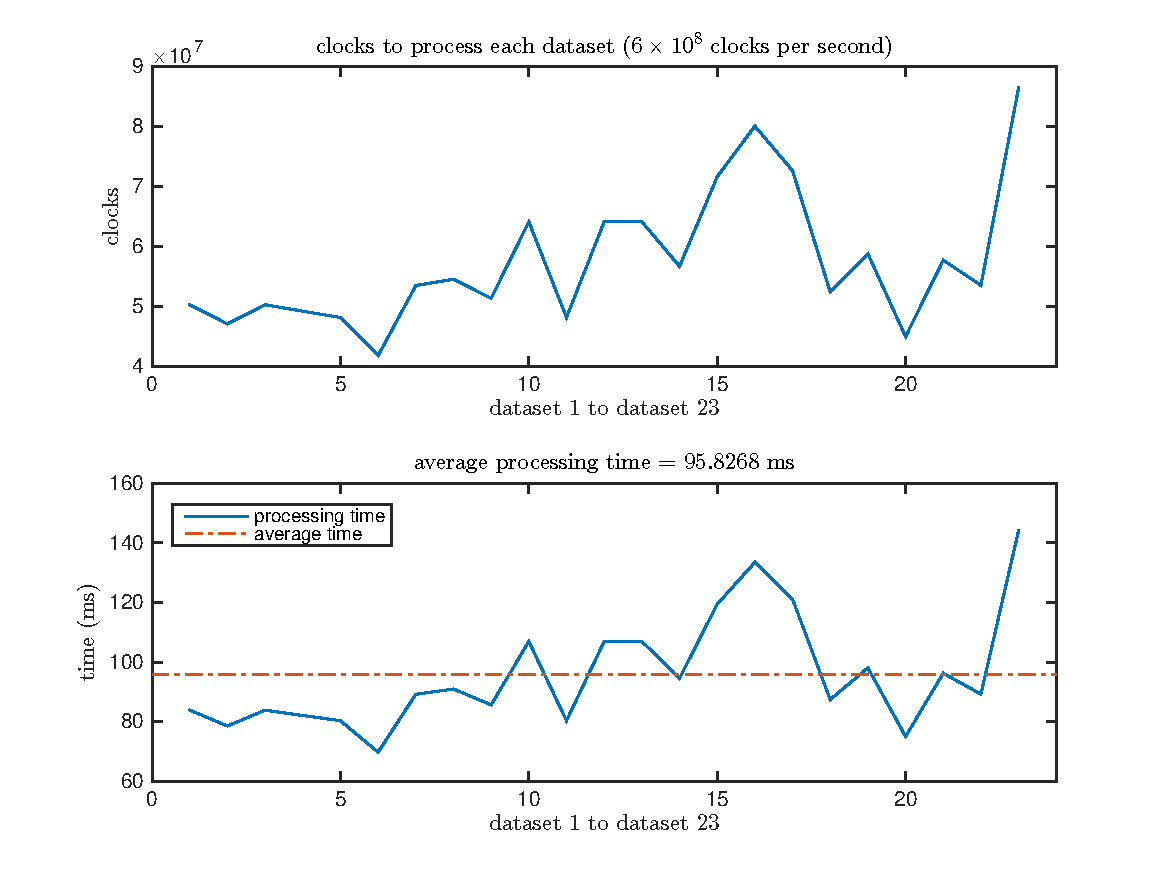
\includegraphics[width=3in, trim={0 0.6cm 0 0.6cm}, clip]{ang/processing_time}
\end{figure}
\end{frame}

%--------------------------------------------
%--------------------------------------------

\begin{frame}
\begin{itemize}
\item Probabilities of 27 words computed by MATLAB (\textcolor{navy_matlab}{navy circle $\circ$})
\item Probabilities of 27 words computed by DSP (\textcolor{orange_matlab}{orange cross $\times$})
\item Dataset 1 has the largest relative error among 23 datasets.
\end{itemize}

\begin{figure}[H]
\centering
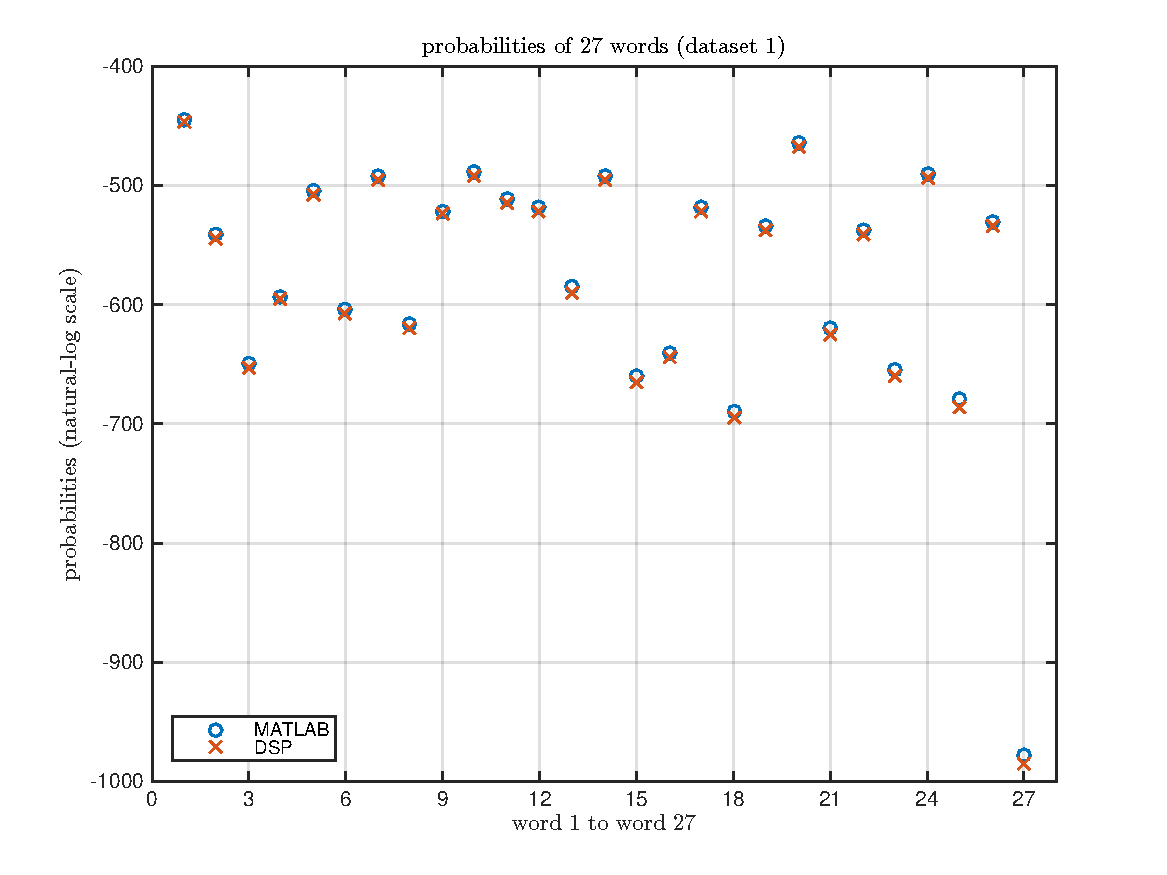
\includegraphics[width=3in, trim={0 0.6cm 0 0.6cm}, clip]{ang/word_probabilities}
\end{figure}
\end{frame}

%----------------------------------------------------------------------------------------
%	Subsection
%----------------------------------------------------------------------------------------

\begin{frame}
\frametitle{Final system implemented on DSP board}
\begin{itemize}
	\item Adaptive noise cancellation based on Least Mean Square Algorithm
	\item Real-time recognition of spoken words
	\item Result indication via a five-LED array
		\begin{itemize}
		\item \LED\offLED\offLED\offLED\offLED\onLED $\longrightarrow$ $(00001)_2 = 1$ $\longrightarrow$ word \textit{one}
		\item \LED\offLED\onLED\onLED\onLED\onLED $\longrightarrow$ $(01111)_2 = 15$ $\longrightarrow$ word \textit{fifteen}
		\item \LED\onLED\offLED\onLED\offLED\onLED $\longrightarrow$ $(10101)_2 = 21$ $\longrightarrow$ word \textit{zero}
		\item \LED\offLED\offLED\offLED\offLED\offLED $\longrightarrow$ $(00000)_2 = 0$ $\longrightarrow$ error
		\end{itemize}
	\item YouTube controller
\end{itemize}
\end{frame}

%----------------------------------------------------------------------------------------
%	Subsection
%----------------------------------------------------------------------------------------

\begin{frame}
\frametitle{Utilization in Home Automation}
\begin{itemize}
	\item Arduino\textsuperscript{\textregistered} board as an intermediate
		\begin{itemize}
		\item the open-source ecosystem of abundant resources already available to Arduino developers
		\item infrared emitter $\longrightarrow$ remote control of TV
		\item WIFI module $\longrightarrow$ wireless communication
		\item relay $\longrightarrow$ AC light switch
		\end{itemize}
\end{itemize}

\begin{figure}[H]
\centering
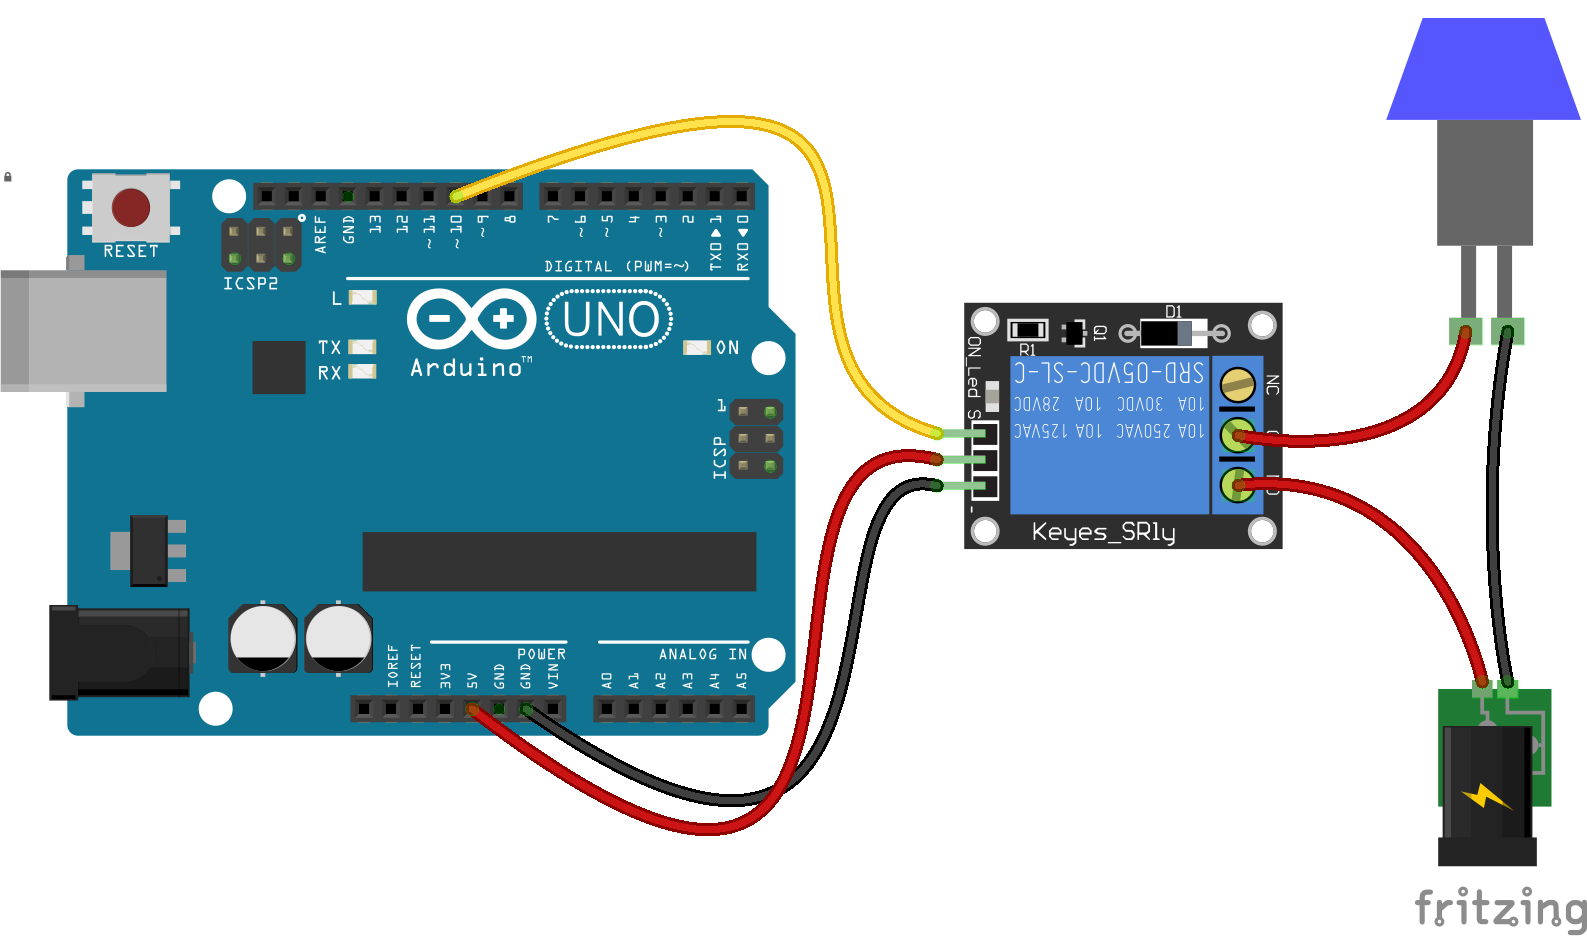
\includegraphics[width=0.5\textwidth]{ang/relay-arduino}
\caption{Control AC Light using Arduino with Relay Module \cite{relay-arduino}}
\end{figure}
\end{frame}

\chapter{Conclusion}

\appendix
\chapter{Appendix}

%----------------------------------------------------------------------------------------
%	Section
%----------------------------------------------------------------------------------------

\section{Speech Signal Processing}

\subsection{Shelving Filter Design}
\label{shelving-appendix}
For gain $G$ in dB, center frequency of transition band $F_c$ in Hz and sampling frequency $F_s$ in Hz, a high-frequency boost second-order shelving filter is represented by following equations \cite{DAFX_book}.

\begin{equation}
y[n] = \frac{1}{a_0} \Big( b_0 x[n] + b_1 x[n-1] + b_2 x[n-3] - a_1 y[n-1] - a_2 y[n-2] \Big)
\end{equation}

\begin{align}
\begin{split}
b_0 &= \frac{V_0 + \sqrt{2V_0} K + K^2}{1 + \sqrt{2} K + K^2}\\
b_1 &= \frac{2 (K^2 - V_0)}{1 + \sqrt{2} K + K^2}\\
b_2 &= \frac{V_0 - \sqrt{2V_0} K + K^2}{1 + \sqrt{2} K + K^2}\\
a_1 &= \frac{2 (K^2 - 1)}{1 + \sqrt{2} K + K^2}\\
a_2 &= \frac{1 - \sqrt{2}K + K^2}{1 + \sqrt{2}K + K^2}
\end{split}
\end{align}
where $a_0 = 1$, $K = \tan(\pi F_c / F_s)$ and $V_0 = 10^{G/20}$.

%--------------------------------------------
%--------------------------------------------

\subsection{Mel-frequency Cepstral Coefficients Extraction}

Table \ref{table:frequency-mel-relationship} shows that $f[m]$ ($m = 0, 1, \dots, M+1$) are equally spaced in mel-scale where $f[0]$ = 0 Hz = 0 mel and $f[21]$ = 8000 Hz = 2835 mel.

\begin{table}[H]
\centering
\caption{Frequency and Mel-scale Relationship}
\label{table:frequency-mel-relationship}
\begin{tabular}{rrr|rrr}
\toprule
m &$f[m]$ in Hz &Mel-scale in mel &m &$f[m]$ in Hz &Mel-scale in mel\\
0  & 0      & 0    & 11 & 1920.4 & 1485\\
1  & 89.2   & 135  & 12 & 2254.5 & 1620\\
2  & 189.9  & 270  & 13 & 2631.2 & 1755\\
3  & 303.3  & 405  & 14 & 3055.9 & 1890\\
4  & 431.3  & 540  & 15 & 3534.7 & 2025\\
5  & 575.5  & 675  & 16 & 4074.7 & 2160\\
6  & 738.1  & 810  & 17 & 4683.4 & 2295\\
7  & 921.5  & 945  & 18 & 5369.8 & 2430\\
8  & 1128.2 & 1080 & 19 & 6143.7 & 2565\\
9  & 1361.3 & 1215 & 20 & 7016.2 & 2700\\
10 & 1624.1 & 1350 & 21 & 8000   & 2835\\
\bottomrule
\end{tabular}
\end{table}

%----------------------------------------------------------------------------------------
%	Section
%----------------------------------------------------------------------------------------

\section{Digital Signal Processor}

\subsection{Fixed-Point Data Types}

\begin{table}[H]
\centering
\caption{Fixed-Point Data Types}
\label{fixed-point-data-types}
\begin{tabu} to \textwidth {XXXX}
\toprule
Type &Size &Min &Max\\
\hline
\texttt{char} &8-bit &-128 &127\\
\hline
\texttt{unsigned char} &8-bit &0 &255\\
\hline
\texttt{short} &16-bit &-32,768 &32,767\\
\hline
\texttt{unsigned short} &16-bit &0 &65,535\\
\hline
\texttt{int} &32-bit &-2,147,483,648 &2,147,483,647\\
\hline
\texttt{unsigned int} &32-bit &0 &4,294,967,295\\
\hline
\texttt{long} &32-bit &-2,147,483,648 &2,147,483,647\\
\hline
\texttt{unsigned long} &32-bit &0 &4,294,967,295\\
\bottomrule
\end{tabu}
\end{table}

\subsection{Floating-Point Data Types}
\label{subsection:float-data-type}

\begin{figure}[H]
\begin{minipage}[t]{0.5\linewidth}
\centering
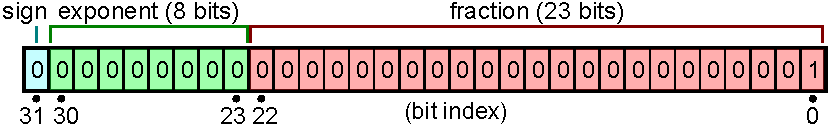
\includegraphics[width=\textwidth]{ang/smallest-denormalized-number}
\caption{Smallest Denormalized Number}
\label{ang/smallest-denormalized-number}
\end{minipage}
\begin{minipage}[t]{0.5\linewidth}
\centering
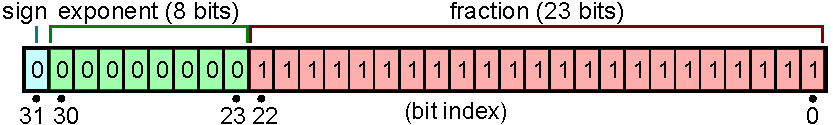
\includegraphics[width=\textwidth]{ang/largest-denormalized-number}
\caption{Largest Denormalized Number}
\label{ang/largest-denormalized-number}
\end{minipage}
\end{figure}

\begin{figure}[H]
\begin{minipage}[t]{0.5\linewidth}
\centering
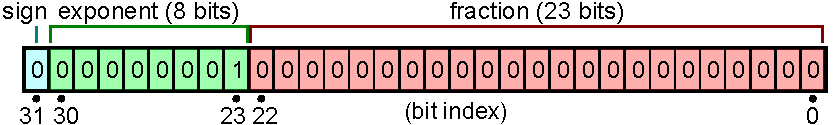
\includegraphics[width=\textwidth]{ang/smallest-normalized-number}
\caption{Smallest Normalized Number}
\label{ang/smallest-normalized-number}
\end{minipage}
\begin{minipage}[t]{0.5\linewidth}
\centering
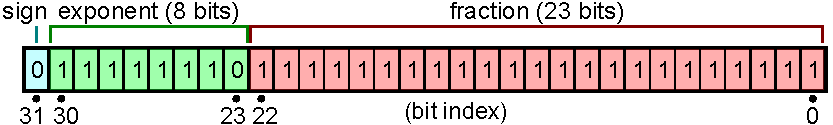
\includegraphics[width=\textwidth]{ang/largest-normalized-number}
\caption{Largest Normalized Number}
\label{ang/largest-normalized-number}
\end{minipage}
\end{figure}

Fig. \ref{ang/smallest-denormalized-number} to Fig. \ref{ang/largest-normalized-number} demonstrate the internal representation of a single-precision floating-point number. The actual mantissa (fraction part) includes 23 fraction bits to the right of the binary point and an \textit{implicit leading bit} to the left of the binary point. When the exponent part is equal to $(00000000)_2$, the implicit leading bit is with value 0 (denormalized); otherwise, the implicit leading bit takes 1 (normalized). Hence, the total length of mantissa is $(23 + 1)$ bits; in other words, \texttt{float} has a precision of $\log_{10}(2^{24}) \approx 7.225$ decimal digits.

\begin{align}
value &=
\begin{cases}
(-1)^{b_{31}} \times (0.b_{22}b_{21} \dots b_{0})_2 \times 2^{- 126} &\text{denormalized}\\
(-1)^{b_{31}} \times (1.b_{22}b_{21} \dots b_{0})_2 \times 2^{(b_{30}b_{29} \dots b_{23})_2 - 127} &\text{normalized}
\end{cases}\\
&=
\begin{cases}
\displaystyle(-1)^{b_{31}} \times \sum_{i=1}^{23} b_{23-i} 2^{-i} \times 2^{- 126} &\text{denormalized}\\
\displaystyle(-1)^{b_{31}} \times ( 1 + \sum_{i=1}^{23} b_{23-i} 2^{-i} ) \times 2^{\sum_{i=0}^{7} b_{i+23} 2^i - 127} &\text{normalized}
\end{cases}
\end{align}

\begin{table}[H]
\centering
\caption{Floating-Point Range}
\label{floating-point-range}
\begin{tabu} to \textwidth {XX}
\toprule
Number &Value\\
\hline
smallest denormalized number &$\pm 2^{-23} \times 2^{-126} \approx \pm 1.4 \times 10^{-45}$\\
\hline
largest denormalized number &$\pm (1-2^{-23}) \times 2^{-126} \approx \pm 1.18 \times 10^{-38}$\\
\hline
smallest normalized number &$\pm 1 \times 2^{-126} \approx \pm 1.18 \times 10^{-38}$\\
\hline
largest normalized number &$\pm (2-2^{-23}) \times 2^{127} \approx \pm 3.4 \times 10^{38}$\\
\bottomrule
\end{tabu}
\end{table}

%----------------------------------------------------------------------------------------
%	Section
%----------------------------------------------------------------------------------------

\section{Design and performance}

\begin{longtable}[c]{|c|c|c|}
\caption {Accuracy of Speaker Dependent System and Speaker Independent System\label{table 3}}\\

\hline
Word & Speaker Dependent System  & Speaker Independent System \\
\hline
\endfirsthead

\hline
Word & Speaker Dependent System  & Speaker Independent System \\
\hline
\endhead

\hline
\endfoot

\hline
\endlastfoot

1& 1 & 0.6\\
\hline
2& 1 &  0.3\\
\hline
3& 1&  0.7\\
\hline
4& 1& 0.3\\
\hline
5& 1& 0.4\\
\hline
6& 1 &  0.6 \\
\hline
7& 1 &   0.2\\
\hline
8& 0.9 &   0.7\\
\hline
9&1 &   0.5\\
\hline
10&1 &  0.8\\
\hline
11& 1 &  0.4\\
\hline
12& 1 &   0.4\\
\hline
13& 1 &   0.5\\
\hline
14& 0.9 & 0.5\\
\hline
15& 1 &  0.3 \\
\hline
16& 1 &  0.5 \\
\hline
17& 1 &  0.2\\
\hline
18& 1 &   0.2\\
\hline
19&0.9& 0.1\\
\hline
20&1 &   0.3\\
\hline
21&1 &  0.5\\
\hline
22& 1 &  0.3\\
\hline
23& 1 &  0.6\\
\hline
24& 1 &   0.4\\
\hline
25& 1 &   0.7\\
\hline
26& 1 &  0.1\\
\hline
27& 0.9 &  0\\
\hline
average & 98.52\% & 41.11\% \\
\end{longtable}


\begin{longtable}[c]{|c|c|c|c|}
\caption{Accuracy of different training data number\label{table 2}}\\

\hline
Word & $\#$ of training data = 20 &$\#$ of training data = 35 &$\#$ of training data = 50 \\
\hline
\endfirsthead

\hline
Word & $\#$ of training data = 20 &$\#$ of training data = 35 &$\#$ of training data = 50 \\
\hline
\endhead

\hline
\endfoot

\hline
\endlastfoot

1& 0.5&0.89 &0.81 \\
\hline
2& 0.5&0.41 &0.60 \\
\hline
3& 0.45& 0.75&0.96 \\
\hline
4& 0.4&0.69 &0.86 \\
\hline
5& 0.5& 0.61& 0.88\\
\hline
6& 0.75& 0.96 &0.96 \\
\hline
7& 0.6&0.62 &0.83 \\
\hline
8& 0.85&0.88 &0.92 \\
\hline
9& 0.35&0.42 &0.60 \\
\hline
10& 0.8& 0.75& 0.91\\
\hline
11& 0.45& 0.58& 0.81\\
\hline
12& 0.55& 0.79&0.88 \\
\hline
13& 0.4&0.38 &0.44 \\
\hline
14& 0.55&0.86 &0.78 \\
\hline
15& 0.4& 0.65&0.70 \\
\hline
16& 0.45&0.48 &0.65 \\
\hline
17& 0.3& 0.31& 0.47\\
\hline
18& 0.2& 0.38&0.78 \\
\hline
19& 0.2& 0.21&0.57 \\
\hline
20& 0.85& 0.79&0.94 \\
\hline
21& 0.6& 0.72& 0.91\\
\hline
22& 0.3& 0.62& 0.57\\
\hline
23& 0.75&0.65 &0.78 \\
\hline
24& 0.55& 0.75&0.81 \\
\hline
25& 0.95&0.98 &0.96 \\
\hline
26& 0.05& 0.24& 0.52\\
\hline
27& 0& 0.08& 0.10\\
\hline
average & 49.07\% & 60.90\% & 74.08\% \\
\end{longtable}

%----------------------------------------------------------------------------------------
%	Section
%----------------------------------------------------------------------------------------

\section{Final Implementation}

\begin{figure}[H]
\centering
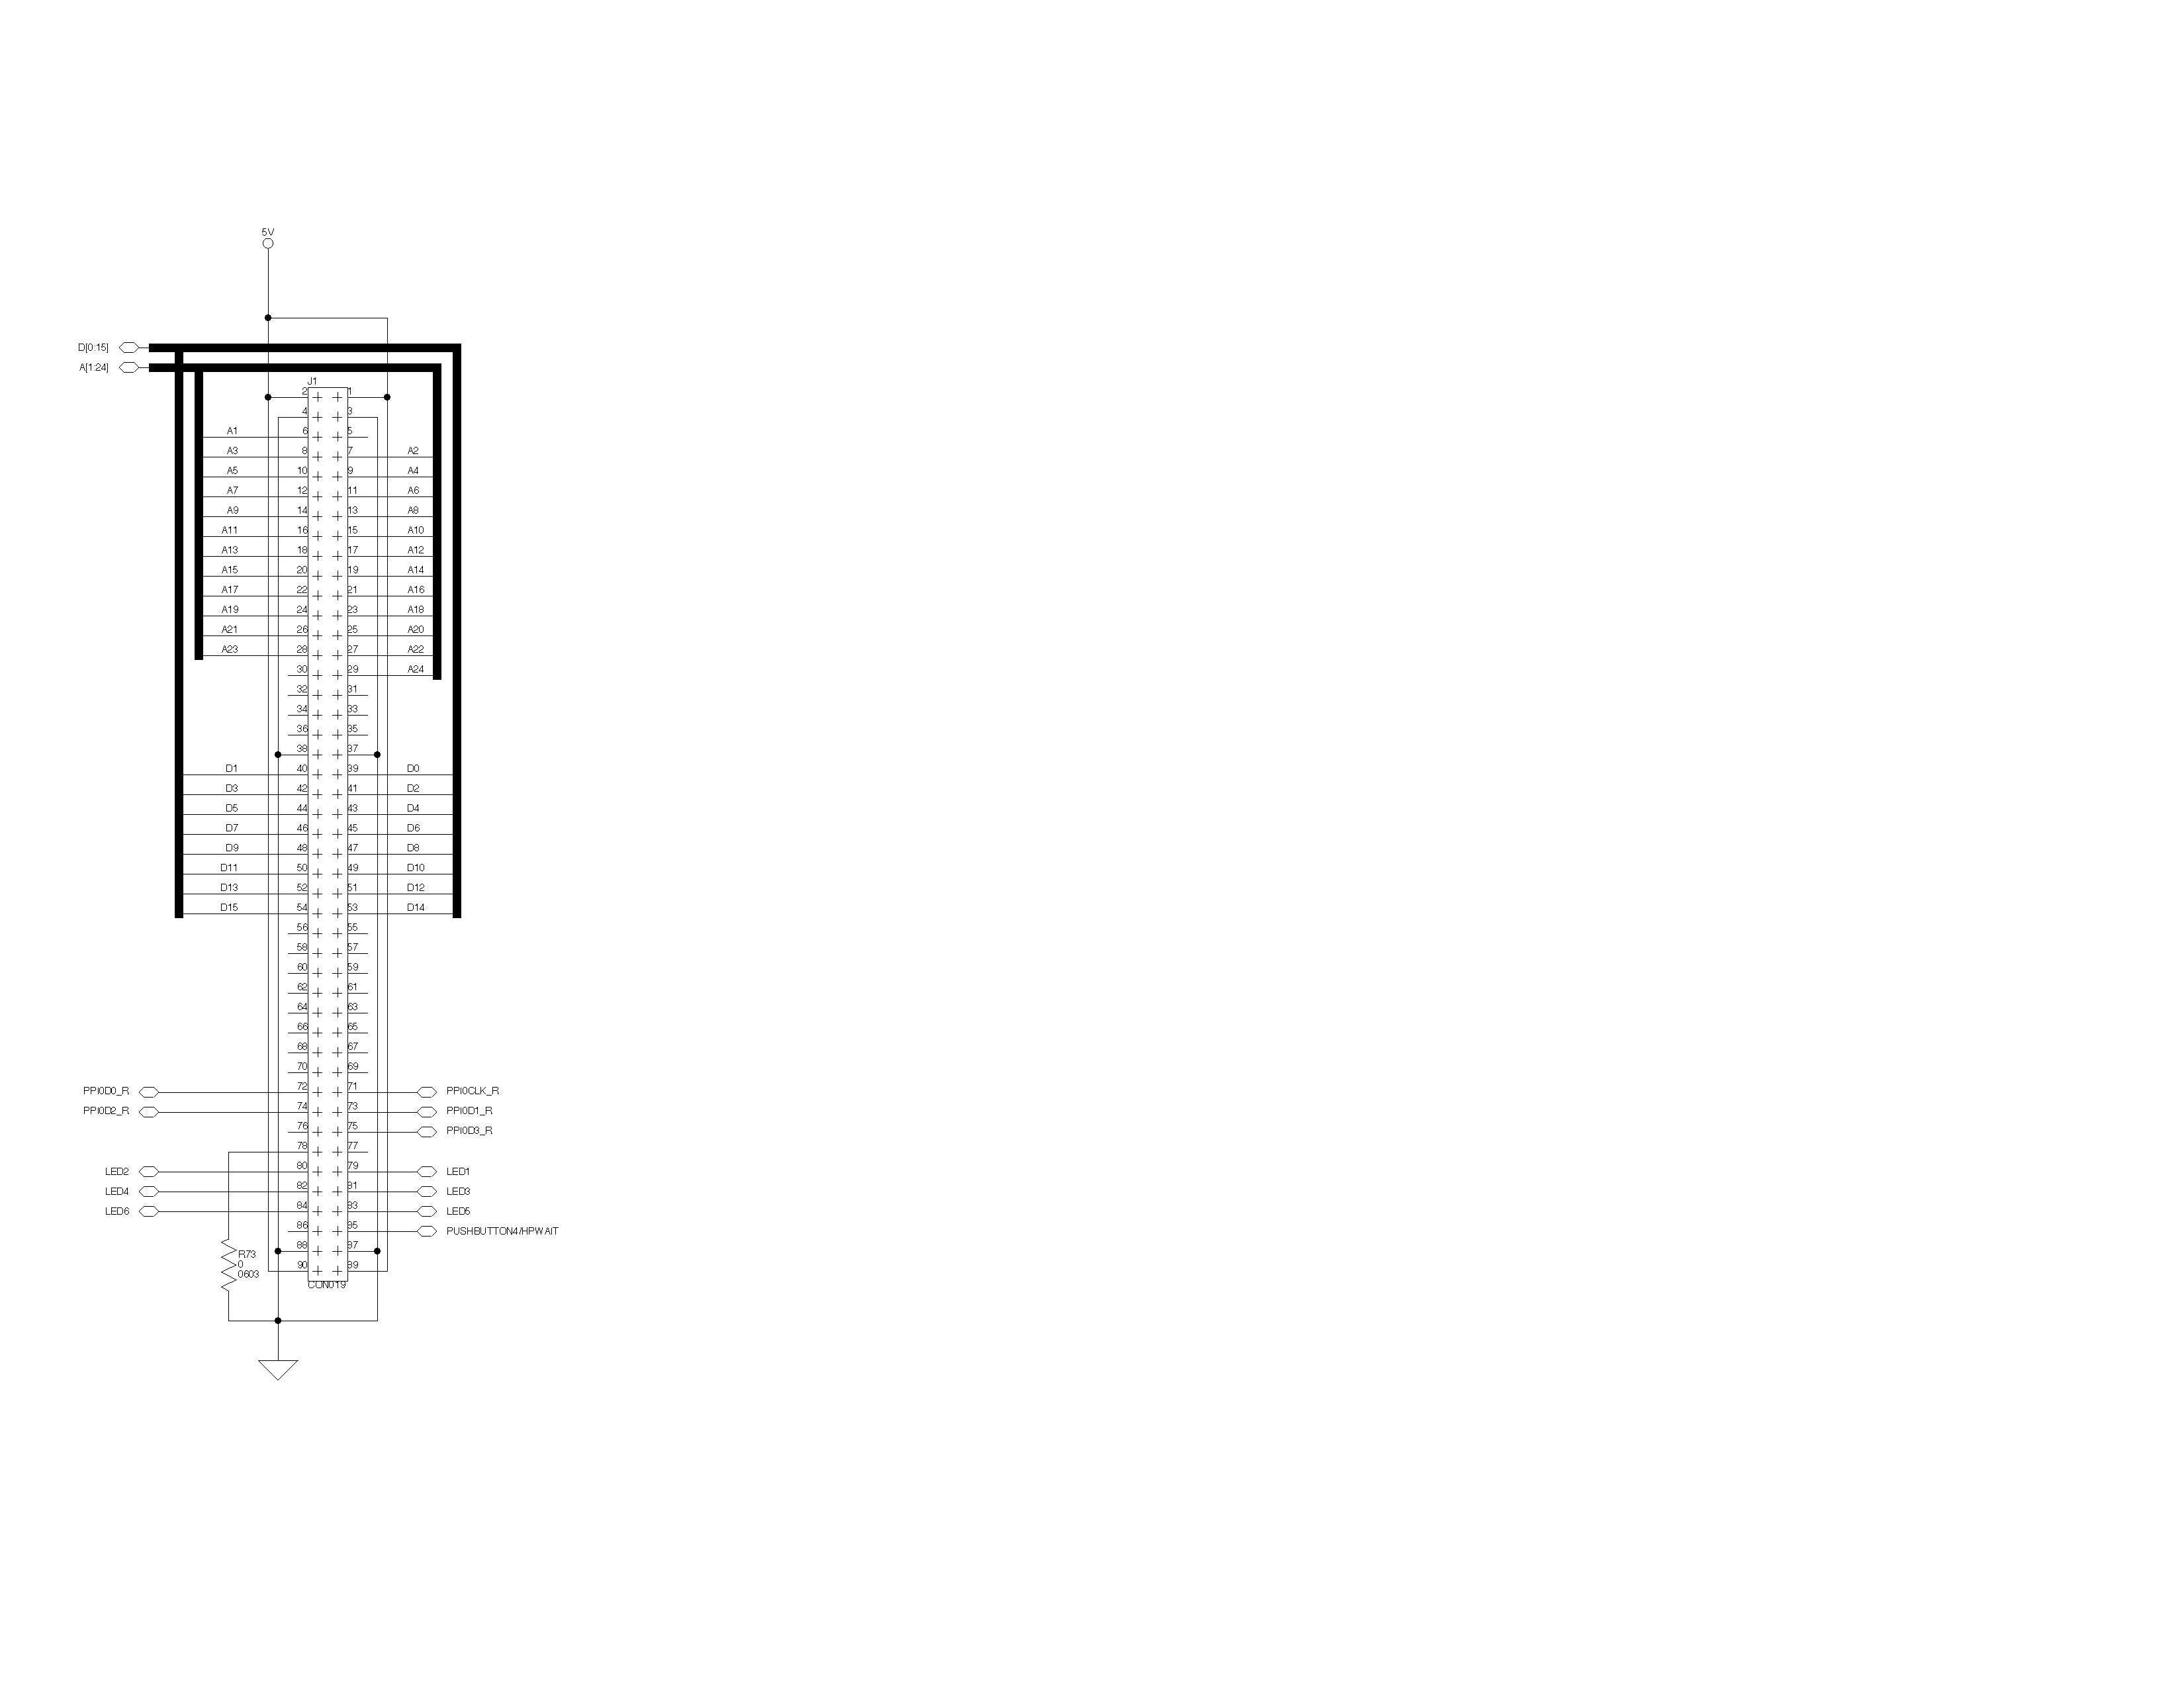
\includegraphics[width=3in]{ang/J1-schematic}
\caption{ADSP-BF548 J1 Connector \cite{bf548-manual}}
\label{J1-schematic}
\end{figure}

\listoffigures
% \bibliography{chapter/bib_zheng,chapter/bib_li,chapter/bib_sun}
\bibliography{chapter/bib_li}
\end{document}
